% 勉強ノート: 自己相互作用のある ALP の超放射と BH のスピン
% ビルド: cd study && latexmk -lualatex study_note.tex
% 前提: 学部の物理(量子力学の水素原子・摂動・Fermi の黄金律、古典力学、特殊相対論)。
%       一般相対論は必要な結果だけを与える。
\documentclass[a4paper,10pt]{ltjsarticle}
\usepackage[margin=22mm,top=22mm,bottom=24mm]{geometry}
\usepackage{amsmath,amssymb,bm}
\usepackage[dvipsnames]{xcolor}
\usepackage{booktabs,tabularx,array,float}
\usepackage{enumitem}
\usepackage[most]{tcolorbox}
\usepackage{tikz}
\usetikzlibrary{arrows.meta,positioning,calc,decorations.pathmorphing,shapes.geometric,patterns}
\usepackage{pgfplots}
\pgfplotsset{compat=1.18}
\usepgfplotslibrary{fillbetween,groupplots}
\usepackage[font=small,labelfont=bf]{caption}
\usepackage[colorlinks=true,breaklinks=true,allcolors=MidnightBlue]{hyperref}

% ---------- 記号 ----------
\newcommand{\Msun}{\ensuremath{\,M_\odot}}
\newcommand{\eV}{\ensuremath{\,\mathrm{eV}}}
\newcommand{\GeV}{\ensuremath{\,\mathrm{GeV}}}
\newcommand{\yr}{\ensuremath{\,\mathrm{yr}}}
\newcommand{\Mpl}{\ensuremath{M_\mathrm{Pl}}}
\newcommand{\dd}{\mathrm{d}}
\newcommand{\rp}{\ensuremath{\tilde r_+}}
\newcommand{\arxiv}[1]{\href{https://arxiv.org/abs/#1}{arXiv:#1}}

% ---------- 配色 ----------
\definecolor{cA}{HTML}{2A78D6}
\definecolor{cB}{HTML}{EB6834}
\definecolor{cC}{HTML}{1BAF7A}
\definecolor{cD}{HTML}{8E5BC9}
\definecolor{cM}{HTML}{8A8984}
\definecolor{ink}{HTML}{0B0B0B}
\definecolor{ink2}{HTML}{52514E}
\definecolor{gridc}{HTML}{E4E3DF}
\pgfplotsset{note/.style={
  axis line style={ink2}, tick style={ink2}, tick label style={font=\scriptsize, color=ink2},
  label style={font=\small, color=ink}, major grid style={gridc}, grid=major, clip=true}}

% ---------- 囲み ----------
\newtcolorbox{summary}[1][]{colback=cA!5, colframe=cA!60, boxrule=0.5pt, arc=2pt, left=5pt, right=5pt, top=3pt, bottom=3pt, fonttitle=\small\bfseries, coltitle=ink, colbacktitle=cA!14, title={まとめ}, #1}
\newtcolorbox{numcheck}[1][]{colback=cC!5, colframe=cC!60, boxrule=0.5pt, arc=2pt, left=5pt, right=5pt, top=3pt, bottom=3pt, fonttitle=\small\bfseries, coltitle=ink, colbacktitle=cC!14, title={数値で確かめる}, #1}
\newtcolorbox{caution}[1][]{colback=cB!5, colframe=cB!70, boxrule=0.5pt, arc=2pt, left=5pt, right=5pt, top=3pt, bottom=3pt, fonttitle=\small\bfseries, coltitle=ink, colbacktitle=cB!15, title={注意}, #1}
\newtcolorbox{tocode}[1][]{colback=cM!6, colframe=cM!60, boxrule=0.4pt, arc=2pt, left=5pt, right=5pt, top=2pt, bottom=2pt, fontupper=\small, #1}

\setlist{itemsep=2pt, topsep=4pt, parsep=0pt}
\numberwithin{equation}{section}

\title{勉強ノート\\回転するブラックホール・超軽量粒子の雲・自己相互作用\\{\large --- GWTC-5 の BH スピンで ALP を調べるための物理 ---}}
\author{}
\date{2026年11月}

\begin{document}
\maketitle
\vspace{-2em}

\begin{tcolorbox}[colback=white, colframe=ink2, boxrule=0.4pt, arc=2pt, left=6pt, right=6pt]
\small
\textbf{このノートについて}
\begin{itemize}
\item 研究(\texttt{Superradiance\_LVKpop})で使った物理を、学部の物理だけを前提に、途中の式を省略せずに導く。
\item 前提にするのは、量子力学(水素原子、摂動、Fermi の黄金律)、古典力学、特殊相対論である。一般相対論は、必要な結果(Kerr 時空の性質、面積定理)だけを与え、意味を説明する。
\item 各節の終わりに「まとめ」を置く。研究ノートのエントリ(E1--E10)とコード(\texttt{research/calc/})との対応は、灰色の枠に書く。
\end{itemize}
\end{tcolorbox}

\tableofcontents
\newpage

% 1. はじめに: 問い、単位、重力の微細構造定数
\section{はじめに: 何を調べるのか}\label{sec:intro}

\subsection{研究の問い}

質量 $\mu\sim10^{-12}\eV$ の非常に軽いスカラー粒子(ALP、axion-like particle)があると、回転するブラックホール(BH)のまわりに、その粒子が非常に多く集まった「雲」ができる。雲は BH の回転のエネルギーと角運動量を吸い取って育つ。そのため、この粒子があれば、ある範囲の質量の BH は速く回っていられない。

重力波の観測(LIGO--Virgo--KAGRA、カタログ GWTC-5)では、合体する BH の質量とスピンが測られている。そこから、この粒子について逆の結論が出ている。
\begin{itemize}
\item 速く回る BH がいるので、この質量の粒子は排除される。
\item BH のスピンが質量ごとにある値に集まっているように見えるので、この質量の粒子がいる証拠がある。
\end{itemize}
研究の問いは、粒子どうしの相互作用(自己相互作用)を入れるとこの二つが両立するか、である。自己相互作用があると、雲が大きく育つ前に飽和し、BH が回転を失う速さが遅くなる。若い BH は回転を保ち、年をとった BH だけが回転を失う、ということが起こりうる。

このノートでは、この問いに答えるのに要る物理を順に導く。
\begin{enumerate}
\item 回転する BH の性質(\S\ref{sec:kerr})
\item BH から回転を取り出す「超放射」の条件(\S\ref{sec:superradiance})
\item BH のまわりの粒子の束縛状態「重力原子」と、その成長率(\S\ref{sec:atom})
\item 雲の成長と BH の回転の減少(\S\ref{sec:cloud})
\item 自己相互作用と、それが起こす準位間の遷移(\S\ref{sec:selfint})
\item 準平衡と、回転を失う速さ(\S\ref{sec:equilibrium})
\item 吸収で回転が戻らないこと(\S\ref{sec:norestore})
\item 合体で生まれる 2 世代目の BH のスピン(\S\ref{sec:secondgen})
\item これらを組み合わせた「窓」(\S\ref{sec:window})
\end{enumerate}

\begin{figure}[H]
\centering
% BH と雲の大きさ(模式図)
\begin{tikzpicture}[scale=1.0]
  % 雲(同心円のぼかし)
  \foreach \r/\o in {3.0/0.05, 2.6/0.08, 2.2/0.11, 1.8/0.14, 1.4/0.12, 1.0/0.08}{
    \fill[cA, opacity=\o] (0,0) ellipse ({\r} and {0.55*\r});
  }
  % BH
  \fill[ink] (0,0) circle (0.12);
  \draw[ink2, thin] (0,0) circle (0.17);
  % 回転の矢印
  \draw[-{Stealth[length=2mm]}, ink2] (0.32,0.1) arc (10:300:0.32 and 0.18);
  % 寸法
  \draw[{Stealth[length=2mm]}-{Stealth[length=2mm]}, ink2] (0,-0.25) -- (2.2,-1.21) node[midway, below right, font=\small, color=ink] {$r_c\simeq r_g/\alpha^2$};
  \node[font=\small, anchor=west] at (0.25,0.45) {BH($r_g$)};
  \node[font=\small, color=cA!80!black] at (2.9,1.45) {粒子の雲};
  \node[font=\scriptsize, color=ink2, align=left, anchor=west] at (3.4,0.2) {$\alpha=0.1$ なら\\$r_c\approx100\,r_g$};
\end{tikzpicture}

\caption{BH と雲の大きさの関係(模式図)。雲の大きさ $r_c\simeq r_g/\alpha^2$ は、$\alpha\sim0.1$ では BH の大きさ $r_g$ の 100 倍ほどになる。雲のごく一部が地平線にかかり、そこで BH と角運動量をやりとりする。}
\label{fig:bhcloud}
\end{figure}

\subsection{単位と記号}

\paragraph{自然単位}
このノートでは、ことわりがない限り $\hbar=c=1$ とする。このとき質量・エネルギー・振動数・長さの逆数はすべて同じ次元をもつ。数値を出すときは次の換算を使う。
\begin{equation}
\hbar=6.582\times10^{-16}\eV\,\mathrm{s},\qquad
\frac{\mu c^2}{\hbar}=1.519\times10^{3}\,\mathrm{s}^{-1}\times\frac{\mu}{10^{-12}\eV}.
\label{eq:hbar}
\end{equation}

\paragraph{BH の尺度}
質量 $M$ の BH は、長さ $r_g$ と時間 $t_g$ の尺度をもつ。
\begin{equation}
r_g\equiv\frac{GM}{c^2}=1.477\,\mathrm{km}\times\frac{M}{M_\odot},\qquad
t_g\equiv\frac{GM}{c^3}=4.925\,\mu\mathrm{s}\times\frac{M}{M_\odot}.
\label{eq:rg}
\end{equation}
$r_g$ を「重力半径」と呼ぶ(Schwarzschild 半径 $2r_g$ の半分)。BH の章(\S\ref{sec:kerr})では、さらに $G=1$ とおき、$M=1$ を長さの単位にすることがある。

\subsection{重力の微細構造定数 $\alpha$}\label{sec:alpha}

この研究のすべての式に現れる無次元量が
\begin{equation}
\alpha\equiv\frac{GM\mu}{\hbar c}
\label{eq:alpha}
\end{equation}
である。意味は三通りに読める。

\paragraph{読み方 1: 二つの長さの比}
粒子の換算 Compton 波長は $\lambda_c=\hbar/(\mu c)$ である。これと重力半径の比をとると
\begin{equation}
\frac{r_g}{\lambda_c}=\frac{GM/c^2}{\hbar/(\mu c)}=\frac{GM\mu}{\hbar c}=\alpha.
\end{equation}
$\alpha\ll1$ なら、粒子の波は BH よりずっと大きい。

\paragraph{読み方 2: 時間の比}
式 \eqref{eq:alpha} は、粒子の振動数 $\mu c^2/\hbar$ と BH の時間 $t_g$ の積でもある。
\begin{equation}
\alpha=\frac{\mu c^2}{\hbar}\times\frac{GM}{c^3}=\frac{\mu c^2}{\hbar}\,t_g.
\label{eq:alpha_time}
\end{equation}
数値は式 \eqref{eq:hbar}、\eqref{eq:rg} から
\begin{equation}
\alpha=1.519\times10^{3}\,\mathrm{s}^{-1}\times4.925\times10^{-6}\,\mathrm{s}\times\frac{M}{M_\odot}\frac{\mu}{10^{-12}\eV}
=0.0748\times\frac{M}{10\,M_\odot}\frac{\mu}{10^{-12}\eV}.
\label{eq:alpha_num}
\end{equation}

\paragraph{読み方 3: 水素原子の $\alpha_\mathrm{em}$ の重力版}
水素原子では、電子(質量 $m_e$)が Coulomb ポテンシャル $V=-e^2/(4\pi\varepsilon_0r)\equiv-\alpha_\mathrm{em}\hbar c/r$ に束縛される。BH のまわりの粒子(質量 $\mu$)は、遠方では Newton のポテンシャル
\begin{equation}
V(r)=-\frac{GM\mu}{r}=-\alpha\frac{\hbar c}{r}
\label{eq:Vgrav}
\end{equation}
に束縛される。$\alpha_\mathrm{em}$ のところに $\alpha$ が入るだけなので、\S\ref{sec:atom} で水素原子の結果をそのまま使える。

\begin{numcheck}
GW241011 の主星($M=19.6\Msun$)と $\mu=0.71\times10^{-12}\eV$ では、式 \eqref{eq:alpha_num} から
\[
\alpha=0.0748\times1.96\times0.71=0.104.
\]
研究ノートの値(E2、E3)と一致する。
\end{numcheck}

\begin{tocode}
コード: \texttt{research/calc/sr.py} の \texttt{alpha\_of(M, mu\_eV)} が式 \eqref{eq:alpha_time} を計算する。定数は \texttt{TSUN} $=GM_\odot/c^3$、\texttt{HBAR\_EVS} $=\hbar$ [eV s]。
\end{tocode}

\begin{summary}
\begin{itemize}
\item 長さの尺度は $r_g=GM/c^2$、時間の尺度は $t_g=GM/c^3$。
\item $\alpha=GM\mu/(\hbar c)=0.0748\,(M/10M_\odot)(\mu/10^{-12}\eV)$ は、BH の大きさと粒子の波長の比であり、重力原子の微細構造定数である。
\end{itemize}
\end{summary}

% 2. 回転するブラックホール
\section{回転するブラックホール}\label{sec:kerr}

この節では、回転する BH(Kerr BH)について、後で使う量を導く。Kerr 時空そのもの(Einstein 方程式の解)は導かず、結果を与える。この節では $G=c=1$ とし、必要なときに単位を戻す。

\subsection{質量・角運動量・スピン}

孤立した BH は、質量 $M$ と角運動量 $J$ の二つの数で決まる(電荷は無視する)。長さの次元をもつ回転のパラメータ $a$ と、無次元のスピン $\chi$ を
\begin{equation}
a\equiv\frac{J}{M},\qquad \chi\equiv\frac{J}{M^2}=\frac{a}{M}
\qquad\Bigl(\text{単位を戻すと } \chi=\frac{cJ}{GM^2}\Bigr)
\label{eq:chi}
\end{equation}
で定義する。$\chi$ が研究で「スピン」と呼んでいる量である。地平線が存在するには $|\chi|\le1$ でなければならない(次の小節)。

\subsection{地平線}

Kerr 時空を Boyer--Lindquist 座標 $(t,r,\theta,\phi)$ で書くと、計量に次の関数が現れる。
\begin{equation}
\Delta(r)\equiv r^2-2Mr+a^2.
\label{eq:Delta}
\end{equation}
$\Delta=0$ となる半径が地平線である。二次方程式 $r^2-2Mr+a^2=0$ を解くと
\begin{equation}
r_\pm=\frac{2M\pm\sqrt{4M^2-4a^2}}{2}=M\pm\sqrt{M^2-a^2}=M\bigl(1\pm\sqrt{1-\chi^2}\bigr).
\label{eq:rpm}
\end{equation}
外側の $r_+$ が事象の地平線である。$|\chi|>1$ では根号の中が負になり、地平線がない。以後
\begin{equation}
\rp\equiv\frac{r_+}{M}=1+\sqrt{1-\chi^2}
\label{eq:rptilde}
\end{equation}
を使う。回転しない BH($\chi=0$)では $\rp=2$(Schwarzschild 半径 $2M$)、最大に回る BH($\chi=1$)では $\rp=1$ である。

\paragraph{よく使う恒等式}
$r_+$ は $\Delta(r_+)=0$ を満たすので、$r_+^2-2Mr_++a^2=0$、すなわち
\begin{equation}
r_+^2+a^2=2Mr_+.
\label{eq:identity}
\end{equation}
これを何度も使う。

\subsection{地平線の角速度 $\Omega_H$}

回転する BH のまわりでは、空間そのものが回転方向に引きずられる(慣性系の引きずり)。地平線上では、どんな観測者も角速度
\begin{equation}
\Omega_H=\frac{a}{r_+^2+a^2}
\label{eq:OmegaH_def}
\end{equation}
で回らざるをえない。これを地平線の角速度と呼ぶ。恒等式 \eqref{eq:identity} を代入すると
\begin{equation}
\Omega_H=\frac{a}{2Mr_+}=\frac{\chi M}{2M\cdot M\rp}=\frac{\chi}{2\rp}\cdot\frac{1}{M}.
\label{eq:OmegaH}
\end{equation}
単位を戻すと $\Omega_H=\dfrac{\chi}{2\rp}\dfrac{c^3}{GM}$ である。

\begin{itemize}
\item $\chi\to0$: $\Omega_H\to0$。
\item $\chi=1$: $\rp=1$ なので $\Omega_H=1/(2M)$。
\item $\chi\ll1$: $\rp\simeq2$ なので $\Omega_H\simeq\chi/(4M)$。
\end{itemize}

\begin{numcheck}
$M=15\Msun$、$\chi=0.69$ では、$\rp=1+\sqrt{1-0.476}=1.724$、$\Omega_H M=0.69/(2\times1.724)=0.200$。$t_g=GM/c^3=74\,\mu\mathrm{s}$ なので $\Omega_H=0.200/74\,\mu\mathrm{s}=2.7\times10^3\,\mathrm{s}^{-1}$。
\end{numcheck}

\subsection{地平線の面積と既約質量}

地平線の面積は
\begin{equation}
A=4\pi(r_+^2+a^2)=8\pi Mr_+=8\pi M^2\rp
\label{eq:area}
\end{equation}
である(2 番目の等号で恒等式 \eqref{eq:identity} を使った)。

面積を「同じ面積をもつ回転しない BH の質量」で表したものを既約質量 $M_\mathrm{irr}$ と呼ぶ。回転しない BH の面積は $4\pi(2M)^2=16\pi M^2$ なので、
\begin{equation}
A\equiv16\pi M_\mathrm{irr}^2
\quad\Longrightarrow\quad
M_\mathrm{irr}^2=\frac{A}{16\pi}=\frac{8\pi M^2\rp}{16\pi}=\frac{M^2\rp}{2}.
\label{eq:Mirr}
\end{equation}

\subsection{Christodoulou の式: 質量 = 既約質量 + 回転のエネルギー}

$M$ を $M_\mathrm{irr}$ と $J$ で表す。$s\equiv\sqrt{1-\chi^2}$ と書くと、$\rp=1+s$ で、式 \eqref{eq:Mirr} は $M_\mathrm{irr}^2=M^2(1+s)/2$ である。次の量を計算する。
\begin{align}
\frac{J^2}{4M_\mathrm{irr}^2}
&=\frac{\chi^2M^4}{4\cdot M^2(1+s)/2}=\frac{\chi^2M^2}{2(1+s)}
=\frac{(1-s^2)M^2}{2(1+s)}=\frac{(1-s)M^2}{2}.
\end{align}
3 番目の等号で $\chi^2=1-s^2$ を使い、最後に $1-s^2=(1-s)(1+s)$ で約分した。これと $M_\mathrm{irr}^2=(1+s)M^2/2$ を足すと
\begin{equation}
M_\mathrm{irr}^2+\frac{J^2}{4M_\mathrm{irr}^2}=\frac{(1+s)M^2}{2}+\frac{(1-s)M^2}{2}=M^2.
\label{eq:christodoulou}
\end{equation}
これが Christodoulou の式である。BH の質量は、取り出せない部分 $M_\mathrm{irr}$ と、回転に蓄えられた部分 $J^2/(4M_\mathrm{irr}^2)$ からなる。

\paragraph{取り出せるエネルギー}
$J$ を 0 まで取り出したとき残る質量は $M_\mathrm{irr}$ である。取り出せるエネルギーは $M-M_\mathrm{irr}=M(1-\sqrt{\rp/2})$ で、$\chi=1$ では $M(1-1/\sqrt2)=0.29M$ になる。超放射の雲は、このエネルギーの一部を吸い取る。

\subsection{面積定理と BH の第一法則}

\paragraph{面積定理}
古典的な過程では、地平線の面積は減らない(Hawking の面積定理)。
\begin{equation}
\dd A\ge0\quad\Longleftrightarrow\quad\dd M_\mathrm{irr}\ge0.
\label{eq:areatheorem}
\end{equation}
これは一般相対論の定理で、ここでは結果として使う。

\paragraph{第一法則}
Christodoulou の式 \eqref{eq:christodoulou} を $M=M(M_\mathrm{irr},J)$ とみて微分すると、BH の第一法則が出る。まず
\begin{equation}
2M\,\dd M=\Bigl(2M_\mathrm{irr}-\frac{J^2}{2M_\mathrm{irr}^3}\Bigr)\dd M_\mathrm{irr}+\frac{2J}{4M_\mathrm{irr}^2}\,\dd J.
\end{equation}
$\dd J$ の係数を $2M$ で割ると
\begin{equation}
\frac{\partial M}{\partial J}=\frac{J}{4MM_\mathrm{irr}^2}=\frac{\chi M^2}{4M\cdot M^2\rp/2}=\frac{\chi}{2\rp M}=\Omega_H
\end{equation}
となり、式 \eqref{eq:OmegaH} の地平線の角速度に一致する。$\dd M_\mathrm{irr}$ の項は、$\dd A=32\pi M_\mathrm{irr}\dd M_\mathrm{irr}$ を使って面積で書き直すと、$(\kappa/8\pi)\dd A$ の形になる($\kappa$ は表面重力、$\kappa=\sqrt{1-\chi^2}/(2r_+)$)。まとめると
\begin{equation}
\dd M=\frac{\kappa}{8\pi}\dd A+\Omega_H\,\dd J,\qquad \kappa\ge0.
\label{eq:firstlaw}
\end{equation}

\paragraph{$\kappa$ の確認}
$\dd M_\mathrm{irr}$ の係数は $(M_\mathrm{irr}-J^2/4M_\mathrm{irr}^3)/M$ である。$\dd M_\mathrm{irr}=\dd A/(32\pi M_\mathrm{irr})$ を代入すると、
\[
\frac{\kappa}{8\pi}=\frac{1}{32\pi M}\Bigl(1-\frac{J^2}{4M_\mathrm{irr}^4}\Bigr),\qquad
\frac{J^2}{4M_\mathrm{irr}^4}=\frac{\chi^2M^4}{M^4\rp^2}=\frac{\chi^2}{\rp^2}
\]
($M_\mathrm{irr}^4=M^4\rp^2/4$ を使った)。$\rp^2-\chi^2=(1+s)^2-(1-s^2)=2s(1+s)=2s\rp$ なので
\[
\kappa=\frac{1}{4M}\cdot\frac{\rp^2-\chi^2}{\rp^2}=\frac{2s\rp}{4M\rp^2}=\frac{\sqrt{1-\chi^2}}{2M\rp}=\frac{\sqrt{1-\chi^2}}{2r_+}.
\]

\begin{summary}
\begin{itemize}
\item 地平線 $r_+=M\rp$、$\rp=1+\sqrt{1-\chi^2}$。地平線の角速度 $\Omega_H=\chi/(2r_+)$。
\item 面積 $A=8\pi M^2\rp=16\pi M_\mathrm{irr}^2$。Christodoulou の式 $M^2=M_\mathrm{irr}^2+J^2/(4M_\mathrm{irr}^2)$。
\item 面積定理 $\dd A\ge0$ と第一法則 $\dd M=(\kappa/8\pi)\dd A+\Omega_H\dd J$。次の節で、この二つから超放射の条件を導く。
\end{itemize}
\end{summary}

\begin{tocode}
コード: \texttt{sr.rplus(chi)} が $\rp$、\texttt{sr.omegaH(chi)} が $\Omega_HM=\chi/(2\rp)$。
\end{tocode}

% 3. 超放射の条件
\section{超放射: 回転から波を増幅する条件}\label{sec:superradiance}

\subsection{第一法則と面積定理から導く}

BH に、振動数 $\omega$、方位量子数 $m$ の波が当たるとする。波は $e^{-i\omega t+im\phi}$ の形で、量子 1 個はエネルギー $\hbar\omega$ と、BH の回転軸まわりの角運動量 $m\hbar$ をもつ。BH がこの波の量子を $\delta N$ 個吸収すると(放出なら $\delta N<0$)、
\begin{equation}
\delta M=\hbar\omega\,\delta N,\qquad \delta J=m\hbar\,\delta N.
\end{equation}
第一法則 \eqref{eq:firstlaw} に代入すると
\begin{equation}
\frac{\kappa}{8\pi}\,\delta A=\delta M-\Omega_H\delta J=\hbar\,\delta N\,(\omega-m\Omega_H).
\label{eq:sr_firstlaw}
\end{equation}
面積定理 $\delta A\ge0$ と $\kappa\ge0$ から、右辺は 0 以上でなければならない。
\begin{equation}
\delta N\,(\omega-m\Omega_H)\ge0.
\end{equation}
\begin{itemize}
\item $\omega>m\Omega_H$ のとき: $\delta N\ge0$。BH は波を吸収できる(ふつうの吸収)。
\item $\omega<m\Omega_H$ のとき: $\delta N\le0$。BH はこの波を吸収できず、量子を放出するしかない。入ってきた波は、より大きな振幅で跳ね返される。
\end{itemize}
後者を超放射と呼ぶ。条件は
\begin{equation}
\boxed{\;0<\omega<m\Omega_H\;}
\label{eq:sr_condition}
\end{equation}
である。このとき BH は質量 $\hbar\omega$ と角運動量 $m\hbar$ を 1 量子ごとに失う。失う質量は回転のエネルギー $J^2/(4M_\mathrm{irr}^2)$ から来るので、既約質量(面積)は減らない。

\paragraph{直観}
回転する物体の上に乗った観測者には、波の振動数は $\omega'=\omega-m\Omega$ に見える(角度 $\phi$ が $\phi'=\phi-\Omega t$ に変わるので、$e^{-i\omega t+im\phi}=e^{-i(\omega-m\Omega)t+im\phi'}$)。$\omega<m\Omega$ では $\omega'<0$ になり、回転系での「吸収」が、静止系では「放出」に見える。回転する円柱が電磁波を増幅する効果(Zel'dovich)と同じ仕組みである。

\subsection{質量のある粒子: 増幅が繰り返される}

質量 $\mu$ の粒子の波は、振動数が $\omega<\mu$ なら無限遠に逃げられず、BH のまわりに束縛される(水素原子の束縛状態と同じ。\S\ref{sec:atom})。束縛された波は BH に何度も当たり、超放射の条件を満たしていれば、当たるたびに増幅される。その結果、波の振幅は指数関数的に育つ。質量が「鏡」の役をする「ブラックホール爆弾」である。

束縛状態では $\omega\simeq\mu$ なので、超放射の条件 \eqref{eq:sr_condition} は $\mu<m\Omega_H$ になる。両辺に $M$ をかけ、式 \eqref{eq:OmegaH} と $\alpha=M\mu$($G=\hbar=c=1$)を使うと
\begin{equation}
\alpha<m\,\Omega_HM=\frac{m\chi}{2\rp}=\frac{m\chi}{2(1+\sqrt{1-\chi^2})}.
\label{eq:sr_alpha}
\end{equation}
右辺は $\chi=1$ で最大値 $m/2$ をとるので、$m=1$ の状態が育つには少なくとも $\alpha<1/2$ が要る。

\subsection{臨界スピン}\label{sec:chic}

BH が回転を失っていくと、やがて式 \eqref{eq:sr_alpha} の等号が成り立ち、超放射が止まる。そのときのスピン $\chi_c$ を求める。
\begin{equation}
m\chi_c=2\alpha\bigl(1+\sqrt{1-\chi_c^2}\bigr).
\end{equation}
根号を一方に集める。
\begin{equation}
m\chi_c-2\alpha=2\alpha\sqrt{1-\chi_c^2}.
\label{eq:chic_step}
\end{equation}
右辺は 0 以上なので、$m\chi_c\ge2\alpha$ が必要である。両辺を 2 乗すると
\begin{align}
m^2\chi_c^2-4m\alpha\chi_c+4\alpha^2&=4\alpha^2(1-\chi_c^2),\\
(m^2+4\alpha^2)\chi_c^2-4m\alpha\chi_c&=0.
\end{align}
$\chi_c\ne0$ の解は
\begin{equation}
\boxed{\;\chi_c=\frac{4m\alpha}{m^2+4\alpha^2}\;}
\label{eq:chic}
\end{equation}
である。これが $m\chi_c\ge2\alpha$ を満たすことは、$m\chi_c-2\alpha=2\alpha(m^2-4\alpha^2)/(m^2+4\alpha^2)\ge0$($\alpha\le m/2$ のとき)で確かめられる。

\begin{table}[H]
\centering\small
\caption{臨界スピン $\chi_c$(式 \ref{eq:chic})。$\alpha$ が大きいほど、BH は多くの回転を残す。}
\label{tab:chic}
\begin{tabular}{@{}lcccccc@{}}
\toprule
$\alpha$ & 0.02 & 0.05 & 0.08 & 0.10 & 0.15 & 0.20 \\
\midrule
$m=1$ & 0.080 & 0.198 & 0.312 & 0.385 & 0.550 & 0.690 \\
$m=2$ & 0.040 & 0.100 & 0.159 & 0.198 & 0.293 & 0.385 \\
\bottomrule
\end{tabular}
\end{table}

\begin{caution}
正確には、束縛状態の振動数は $\omega=E_{n\ell m}$ で、$\mu$ より少し小さい($E\simeq\mu(1-\alpha^2/2n^2)$、\S\ref{sec:atom})。研究のコードでは $m\Omega_H=E_{n\ell m}$ を数値的に解いている(\texttt{si.chi\_threshold\_211})。$\alpha=0.104$ での差は $\chi_c$ で $5\times10^{-4}$ ほどで、式 \eqref{eq:chic} で十分よい。
\end{caution}

\begin{summary}
\begin{itemize}
\item 面積定理と第一法則から、$\omega<m\Omega_H$ の波は BH に吸収されず増幅される(超放射)。
\item 質量のある粒子の束縛状態($\omega\simeq\mu$)は繰り返し増幅されて指数関数的に育つ。
\item 成長は BH のスピンが臨界値 $\chi_c=4m\alpha/(m^2+4\alpha^2)$ まで下がると止まる。
\end{itemize}
\end{summary}

% 4. 重力原子
\section{重力原子: BH のまわりの束縛状態}\label{sec:atom}

\subsection{Klein--Gordon 方程式から Schr\"odinger 方程式へ}

質量 $\mu$ の実スカラー場 $\varphi$ は、平坦な時空では Klein--Gordon 方程式
\begin{equation}
\partial_t^2\varphi-\nabla^2\varphi+\mu^2\varphi=0
\label{eq:KG}
\end{equation}
に従う($\hbar=c=1$)。平面波 $e^{-i\omega t+i\bm k\cdot\bm x}$ を入れると $\omega^2=k^2+\mu^2$ で、特殊相対論のエネルギーと運動量の関係そのものである。

\paragraph{弱い重力場}
BH から遠いところ($r\gg M$)では、重力は Newton のポテンシャル $\Phi=-M/r$($G=1$)で表せ、計量は
\begin{equation}
\dd s^2\simeq(1+2\Phi)\,\dd t^2-(1-2\Phi)\,\dd\bm x^2
\end{equation}
である。このとき Klein--Gordon 方程式は、$|\Phi|\ll1$ の 1 次までで
\begin{equation}
(1-2\Phi)\,\partial_t^2\varphi-(1+2\Phi)\nabla^2\varphi+\mu^2\varphi=0
\label{eq:KG_weak}
\end{equation}
になる(計量の逆数 $g^{tt}\simeq1-2\Phi$、$g^{ij}\simeq-(1+2\Phi)\delta^{ij}$ を使った。波動演算子 $(-g)^{-1/2}\partial_\mu(\sqrt{-g}\,g^{\mu\nu}\partial_\nu)$ の $\sqrt{-g}$ は、$\sqrt{-g}\,g^{ij}=-\delta^{ij}+O(\Phi^2)$ なので $\Phi$ の 1 次では効かない)。

\paragraph{速い振動を分ける}
束縛された粒子は非相対論的で、エネルギーはほぼ静止質量 $\mu$ である。そこで、場を速い振動 $e^{-i\mu t}$ とゆっくり変わる複素関数 $\psi(t,\bm x)$ に分ける。
\begin{equation}
\varphi=\frac{1}{\sqrt{2\mu}}\Bigl(\psi\,e^{-i\mu t}+\psi^*e^{i\mu t}\Bigr).
\label{eq:nr_ansatz}
\end{equation}
時間微分は
\begin{equation}
\partial_t^2\bigl(\psi e^{-i\mu t}\bigr)=\bigl(\ddot\psi-2i\mu\dot\psi-\mu^2\psi\bigr)e^{-i\mu t}.
\end{equation}
式 \eqref{eq:KG_weak} に入れて $e^{-i\mu t}$ の係数を集めると($e^{+i\mu t}$ の項は複素共役で同じ式を与える)
\begin{equation}
(1-2\Phi)\bigl(\ddot\psi-2i\mu\dot\psi-\mu^2\psi\bigr)-(1+2\Phi)\nabla^2\psi+\mu^2\psi=0.
\end{equation}
$\mu^2\psi$ の項は、$-(1-2\Phi)\mu^2\psi+\mu^2\psi=2\Phi\mu^2\psi$ にまとまる。残りの項の大きさを比べる。$\psi$ は $E-\mu\sim\mu v^2$ の速さで変わり、$|\Phi|\sim v^2$ なので、
\begin{itemize}
\item $\ddot\psi\sim\mu^2v^4\psi$ は $\mu\dot\psi\sim\mu^2v^2\psi$ より $v^2$ 倍小さい。
\item $\Phi\mu\dot\psi$、$\Phi\nabla^2\psi$ は $\mu^2v^4\psi$ の大きさで、やはり $v^2$ 倍小さい。
\end{itemize}
これらを落とすと
\begin{equation}
-2i\mu\dot\psi+2\Phi\mu^2\psi-\nabla^2\psi=0
\quad\Longrightarrow\quad
i\dot\psi=-\frac{\nabla^2}{2\mu}\psi+\mu\Phi\,\psi.
\end{equation}
$\mu\Phi=-M\mu/r=-\alpha/r$ なので
\begin{equation}
\boxed{\;i\frac{\partial\psi}{\partial t}=\Bigl(-\frac{\nabla^2}{2\mu}-\frac{\alpha}{r}\Bigr)\psi\;}
\label{eq:schrodinger}
\end{equation}
となる。これは水素原子の Schr\"odinger 方程式で、電子の質量 $m_e$ を $\mu$ に、$\alpha_\mathrm{em}$ を $\alpha$ に置き換えたものである。

\paragraph{規格化: $|\psi|^2$ は粒子の数密度}
式 \eqref{eq:nr_ansatz} の係数 $1/\sqrt{2\mu}$ は、$\int|\psi|^2\dd^3x$ が粒子の数 $N$ になるように選んである。実際、$\psi=|\psi|e^{i\theta}$ と書くと $\varphi=\sqrt{2/\mu}\,|\psi|\cos(\mu t-\theta)$ で、時間平均は $\langle\varphi^2\rangle=|\psi|^2/\mu$。速く振動する場のエネルギー密度は $\rho=\tfrac12\langle\dot\varphi^2\rangle+\tfrac12\mu^2\langle\varphi^2\rangle\simeq\mu^2\langle\varphi^2\rangle=\mu|\psi|^2$ なので、数密度は $\rho/\mu=|\psi|^2$ である。

\subsection{水素原子の結果}

式 \eqref{eq:schrodinger} の束縛状態は、水素原子とまったく同じである。
\begin{itemize}
\item \textbf{Bohr 半径}: $r_B=\dfrac{1}{\mu\alpha}$。$\alpha=M\mu$ を使うと $r_B=\dfrac{M}{\alpha^2}$、すなわち $r_B=r_g/\alpha^2$(\S\ref{sec:intro} の図~\ref{fig:bhcloud})。
\item \textbf{エネルギー}(静止質量を含める): $E_n=\mu-\dfrac{\mu\alpha^2}{2n^2}=\mu\Bigl(1-\dfrac{\alpha^2}{2n^2}\Bigr)$。
\item \textbf{量子数}: 主量子数 $n\ge1$、軌道角運動量 $\ell\le n-1$、方位量子数 $|m|\le\ell$。状態を $|n\ell m\rangle$ と書く。
\item \textbf{原点の近く}: 動径関数は $R_{n\ell}(r)\propto r^\ell$($r\ll r_B$)。$\ell$ が大きいほど、波は原点(BH)の近くに来ない。
\end{itemize}
超放射の条件 $\omega<m\Omega_H$ には $m\ge1$ が要る。$m\ge1$ には $\ell\ge1$、$\ell\ge1$ には $n\ge2$ が要るので、最も育ちやすいのは $|211\rangle$ である($\ell$ が最小で BH に最も近づく)。次が $|322\rangle$、その次が $|433\rangle$ である。

\begin{figure}[H]
\centering
% 重力原子の準位(模式図)
\begin{tikzpicture}[x=1cm,y=1cm]
  % 連続状態
  \fill[cM!15] (-0.2,4.6) rectangle (6.4,5.3);
  \draw[ink2, thick] (-0.2,4.6) -- (6.4,4.6) node[right, font=\small] {$E=\mu$};
  \node[font=\scriptsize, color=ink2] at (3.1,5.0) {連続状態(無限遠に逃げられる)};
  % 準位: y = 4.6 - 3.6/n^2
  \foreach \n/\y in {1/1.0, 2/3.10, 3/3.75, 4/4.20}{
    \node[font=\small, anchor=east] at (-0.3,\y) {$n=\n$};
  }
  % l = 0,1,2,3 の列
  \foreach \l/\x in {0/0.4, 1/2.0, 2/3.6, 3/5.2}{
    \node[font=\small] at (\x+0.4,0.3) {$\ell=\l$};
  }
  \draw[ink, line width=0.9pt] (0.0,1.0) -- (0.8,1.0) node[midway, above, font=\scriptsize] {100};
  \draw[ink, line width=0.9pt] (0.0,3.10) -- (0.8,3.10) node[midway, below, font=\scriptsize] {200};
  \draw[cA, line width=1.6pt] (1.6,3.10) -- (2.4,3.10) node[midway, below, font=\scriptsize, color=cA] {211};
  \draw[ink, line width=0.9pt] (0.0,3.75) -- (0.8,3.75);
  \draw[ink, line width=0.9pt] (1.6,3.75) -- (2.4,3.75);
  \draw[cB, line width=1.6pt] (3.2,3.75) -- (4.0,3.75) node[midway, below, font=\scriptsize, color=cB] {322};
  \draw[ink, line width=0.9pt] (0.0,4.20) -- (0.8,4.20);
  \draw[ink, line width=0.9pt] (1.6,4.20) -- (2.4,4.20);
  \draw[ink, line width=0.9pt] (3.2,4.20) -- (4.0,4.20);
  \draw[cD, line width=1.6pt] (4.8,4.20) -- (5.6,4.20) node[midway, below, font=\scriptsize, color=cD] {433};
  % 注記
  \draw[-{Stealth[length=2mm]}, ink2] (6.0,1.0) -- (6.0,4.5);
  \node[font=\scriptsize, color=ink2, align=left, anchor=west] at (6.1,2.6) {束縛エネルギー\\$\mu\alpha^2/2n^2$};
  \node[font=\scriptsize, color=ink2, align=center] at (2.6,2.0) {超放射で育つのは $m\ge1$\\(色の付いた $m=\ell$ の準位)};
\end{tikzpicture}

\caption{重力原子の準位(模式図、間隔は誇張)。エネルギーは静止質量 $\mu$ のすぐ下に並ぶ。超放射で育つのは $m\ge1$ の準位で、最も速いのが $|211\rangle$。$E>\mu$ は無限遠に逃げられる連続状態。}
\label{fig:levels}
\end{figure}

\paragraph{微細構造}
相対論の補正と BH の回転は、水素原子と同じように準位を少しずらす。$\alpha^5$ までの結果は(\arxiv{1908.10370} の式 2.28--2.29)
\begin{equation}
\frac{E_{n\ell m}}{\mu}=1-\frac{\alpha^2}{2n^2}-\frac{\alpha^4}{8n^4}+\frac{f_{n\ell}}{n^3}\alpha^4+\frac{h_\ell}{n^3}\chi m\alpha^5,
\quad f_{n\ell}=-\frac{6}{2\ell+1}+\frac{2}{n},\quad h_\ell=\frac{16}{2\ell(2\ell+1)(2\ell+2)}.
\label{eq:fine}
\end{equation}
$\alpha^4$ の項が相対論の補正(水素原子の微細構造にあたる)、$\chi m\alpha^5$ の項が回転による分裂(超微細構造にあたる)である。このノートの議論では、ほとんど第 2 項までで足りる。

\subsection{なぜ束縛状態が育つのか: 地平線での境界条件}

水素原子では原点で波が正則であることを課す。BH では代わりに、地平線で波が「入っていくだけ」であることを課す(地平線の内側からは何も出てこない)。この境界条件のもとでは、固有振動数が複素数になる。
\begin{equation}
\omega=E+i\Gamma,\qquad \psi\propto e^{-i\omega t}=e^{-iEt}\,e^{\Gamma t}.
\label{eq:complexomega}
\end{equation}
$\Gamma>0$ なら振幅が育ち、$\Gamma<0$ なら減衰する。\S\ref{sec:superradiance} の議論から、$\Gamma$ の符号は $m\Omega_H-E$ の符号と同じである。

\subsection{成長率の大きさ: 見積もり}

$\Gamma$ の大きさを、「地平線を通る粒子の流れ $\div$ 雲の粒子の数」として見積もる。
\begin{enumerate}
\item \textbf{地平線での密度}: 原点の近くで $R_{n\ell}\propto r^\ell$ なので、規格化された波の地平線での密度は
\[
\frac{|\psi(r_+)|^2}{N}\sim\frac{1}{r_B^3}\Bigl(\frac{r_+}{r_B}\Bigr)^{2\ell}.
\]
\item \textbf{流れ}: 地平線と一緒に回る系では波の振動数は $\omega-m\Omega_H$ で、粒子の流れはこれに比例する。流れの大きさは、面積 $\sim r_+^2$、振動数 $(\omega-m\Omega_H)$、場の振幅の 2 乗 $|\varphi|^2\sim|\psi|^2/\mu$ の積の程度である。符号まで含めて
\[
\frac{\dd N}{\dd t}\sim r_+^2\,(m\Omega_H-\omega)\,\frac{|\psi(r_+)|^2}{\mu}.
\]
\item \textbf{率}: $N$ で割り、$r_B=1/(\mu\alpha)$、$r_+\sim M$ を代入する。
\begin{align}
\Gamma\sim\frac{1}{N}\frac{\dd N}{\dd t}
&\sim(m\Omega_H-\omega)\,\frac{r_+^{2\ell+2}}{\mu\,r_B^{2\ell+3}}
=(m\Omega_H-\omega)\,\frac{M^{2\ell+2}(\mu\alpha)^{2\ell+3}}{\mu}\notag\\
&=(m\Omega_H-\omega)\,(M\mu)^{2\ell+2}\alpha^{2\ell+3}
=(m\Omega_H-\omega)\,\alpha^{4\ell+5}.
\label{eq:gamma_estimate}
\end{align}
\end{enumerate}
成長率は $\alpha^{4\ell+5}$ に比例する。$\ell$ が 1 増えるごとに $\alpha^4$ 倍遅くなる。ただし数値の係数も小さくなる(次の小節の $C_{n\ell}$ で $C_{32}/C_{21}=2.2\times10^{-4}$)。両方を合わせると、$\alpha=0.1$ では $|322\rangle$ は $|211\rangle$ より $4$--$7\times10^{-7}$ 倍遅い($\chi=0.5$--$0.9$、研究ノート E4 の相対論的な率)。

\subsection{正確な式と、振幅の率と粒子数の率}

漸近展開の接続による正確な結果は(\arxiv{1908.10370} の式 2.32--2.34、$G=c=\hbar=1$)
\begin{gather}
\Gamma_{n\ell m}=2\rp\,C_{n\ell}\,g_{\ell m}\,(m\Omega_H-E_{n\ell m})\,\alpha^{4\ell+5},
\label{eq:bcst}\\
C_{n\ell}=\frac{2^{4\ell+1}(n+\ell)!}{n^{2\ell+4}(n-\ell-1)!}\Bigl[\frac{\ell!}{(2\ell)!\,(2\ell+1)!}\Bigr]^2,\qquad
g_{\ell m}=\prod_{k=1}^{\ell}\Bigl[k^2(1-\chi^2)+(\chi m-2r_+E_{n\ell m})^2\Bigr]
\notag
\end{gather}
で、見積もり \eqref{eq:gamma_estimate} と同じ形をしている。

\paragraph{$|211\rangle$ の小さい $\alpha$ の極限}
$n=2$、$\ell=m=1$ を代入する。
\begin{equation}
C_{21}=\frac{2^5\cdot3!}{2^6\cdot0!}\Bigl[\frac{1!}{2!\cdot3!}\Bigr]^2=\frac{32\cdot6}{64}\cdot\frac{1}{144}=\frac{3}{144}=\frac{1}{48}.
\end{equation}
$\alpha\to0$ では $r_+E\simeq\rp\alpha\to0$ なので、$g_{11}\to(1-\chi^2)+\chi^2=1$。また $\Omega_H=\chi/(2\rp M)$、$E\simeq\mu=\alpha/M$ から
\begin{equation}
2\rp(\Omega_H-E)\simeq2\rp\Bigl(\frac{\chi}{2\rp M}-\frac{\alpha}{M}\Bigr)=\frac{\chi-2\alpha\rp}{M}.
\end{equation}
これらを式 \eqref{eq:bcst} に入れ、$\alpha^9/M=\alpha^8\mu$ を使うと
\begin{equation}
\Gamma_{211}\simeq\frac{1}{48}\,\frac{\chi-2\alpha\rp}{M}\,\alpha^9=\frac{\mu\,\alpha^8}{48}\bigl(\chi-2\alpha\rp\bigr).
\label{eq:gamma211}
\end{equation}
$\chi-2\alpha\rp=0$ は $\Omega_HM=\alpha$、すなわち $m=1$ の超放射の条件の境目である(\S\ref{sec:chic})。

\paragraph{振幅の率と粒子数の率}
式 \eqref{eq:complexomega} のとおり、$\Gamma$ は場の振幅の成長率である。粒子の数は $N\propto|\psi|^2\propto e^{2\Gamma t}$ で育つので、粒子数の成長率は
\begin{equation}
\Gamma_N\equiv\frac{1}{N}\frac{\dd N}{\dd t}=2\Gamma\simeq\frac{\mu\,\alpha^8}{24}\bigl(\chi-2\alpha\rp\bigr)
\label{eq:gammaN}
\end{equation}
である。

\begin{caution}
文献によって $\Gamma$ が振幅の率か粒子数の率かが違い、2 倍の食い違いが生じやすい。最初の解析(Detweiler 1980)は振幅の率を $1/24$ としたが、これは 2 倍大きすぎ、のちに $1/48$ に訂正された。研究ではすべて粒子数の率 $\Gamma_N=2\Gamma$ を使う(\texttt{sr.NORM\_N = 2})。
\end{caution}

\begin{numcheck}
$M=15\Msun$、$\mu=7\times10^{-13}\eV$、$\chi=0.69$ では、$\alpha=0.0786$、$\rp=1.724$、$\chi-2\alpha\rp=0.419$。
\begin{itemize}
\item 小さい $\alpha$ の式 \eqref{eq:gammaN}: $\Gamma_N/\mu=\alpha^8\times0.419/24$。$\alpha^8=(0.0786)^8=1.46\times10^{-9}$ なので $2.54\times10^{-11}$。
\item $g_{11}$ を入れると: $g_{11}=(1-0.476)+(0.69-2\times1.724\times0.0786)^2=0.524+0.176=0.700$ なので、$\Gamma_N/\mu=1.78\times10^{-11}$。研究の値(E2: $1.776\times10^{-11}$)と一致する。
\item $\mu=7\times10^{-13}\eV$ は $1.06\times10^3\,\mathrm{s}^{-1}$ なので、$\Gamma_N=1.89\times10^{-8}\,\mathrm{s}^{-1}$。粒子数が $e$ 倍になる時間は $1/\Gamma_N=5.3\times10^7\,\mathrm{s}=1.7$ 年。
\end{itemize}
\end{numcheck}

\paragraph{相対論的な補正}
式 \eqref{eq:bcst} は $\alpha$ の小さい極限の式である。研究では、Kerr 時空の Klein--Gordon 方程式を Leaver の連分数法で数値的に解いて比べた(E4、付録~\ref{app:leaver})。$\alpha\lesssim0.08$ では 10\% 以内で合い、$\alpha=0.2$($\chi=0.9$)では解析式が 1.5 倍小さい。窓に効く $\alpha\lesssim0.15$ では、補正は結論を変えない。

\begin{summary}
\begin{itemize}
\item 弱い重力場の Klein--Gordon 方程式は、$\varphi=(2\mu)^{-1/2}(\psi e^{-i\mu t}+\mathrm{c.c.})$ とおくと水素原子の Schr\"odinger 方程式($\alpha_\mathrm{em}\to\alpha$)になる。$|\psi|^2$ は粒子の数密度。
\item 準位 $E_n=\mu(1-\alpha^2/2n^2)$、Bohr 半径 $r_B=r_g/\alpha^2$。最も速く育つのは $|211\rangle$。
\item 地平線の境界条件で振動数が複素数になり、成長率は $\Gamma\propto(m\Omega_H-E)\alpha^{4\ell+5}$。$|211\rangle$ の粒子数の率は $\Gamma_N\simeq\mu\alpha^8(\chi-2\alpha\rp)/24$。
\end{itemize}
\end{summary}

\begin{tocode}
コード: \texttt{sr.omega\_over\_mu} が式 \eqref{eq:fine}、\texttt{sr.gamma\_over\_mu} が式 \eqref{eq:bcst}(振幅の率、\texttt{norm=2} で粒子数の率)、\texttt{sr.gamma\_rel\_over\_mu} が連分数法の表から引いた相対論的な率。
\end{tocode}

% 5. 雲の成長と BH の回転の減少(自由場)
\section{雲の成長と BH の回転の減少(自由場)}\label{sec:cloud}

この節では自己相互作用を入れず(自由場)、$|211\rangle$ の雲が育って BH の回転を奪う過程を追う。

\subsection{雲と BH の連立方程式}

雲の粒子数を $N$ とする。粒子 1 個が BH から角運動量 $m\hbar$($|211\rangle$ では $\hbar$)とエネルギー $\hbar\omega$ を持ち去るので
\begin{equation}
\frac{\dd N}{\dd t}=\Gamma_N(\chi)\,N,\qquad
\frac{\dd J}{\dd t}=-m\hbar\,\Gamma_N N,\qquad
\frac{\dd M}{\dd t}=-\hbar\omega\,\Gamma_N N.
\label{eq:cloud_ode}
\end{equation}
$\Gamma_N$ は BH のスピンの関数で、臨界スピン $\chi_c$ で 0 になる。

\paragraph{粒子数をスピンの単位で数える}
$J=\chi GM^2/c$ なので、角運動量を $\hbar$ で数えると
\begin{equation}
\frac{J}{\hbar}=\chi\,\frac{GM^2}{\hbar c}=\chi\Bigl(\frac{M}{\Mpl}\Bigr)^2,\qquad
\Mpl=\sqrt{\frac{\hbar c}{G}}=2.18\times10^{-8}\,\mathrm{kg}.
\end{equation}
$M=M_\odot$ では $(M_\odot/\Mpl)^2=(1.99\times10^{30}/2.18\times10^{-8})^2=8.3\times10^{75}$ である。そこで粒子数を
\begin{equation}
\varepsilon\equiv\frac{N}{GM^2/(\hbar c)}
\label{eq:epsilon}
\end{equation}
で数えると、$|211\rangle$ では $\dd\chi=-\dd\varepsilon$(質量の変化を無視したとき)になる。BH が $\chi_0$ から $\chi_c$ まで回転を失うと、雲には $\varepsilon=\chi_0-\chi_c$ の粒子がたまる。

\subsection{飽和までの時間}

雲は 1 個の量子(量子ゆらぎ)から育つ。$\Gamma_N$ が一定なら $N(t)=e^{\Gamma_Nt}$ で、飽和の粒子数
\begin{equation}
N_\mathrm{sat}=\frac{\Delta J}{m\hbar}=\frac{(\chi_0-\chi_c)}{m}\Bigl(\frac{M}{\Mpl}\Bigr)^2
\end{equation}
に届く時間は
\begin{equation}
t_\mathrm{sat}\simeq\frac{\ln N_\mathrm{sat}}{\Gamma_N}.
\label{eq:tsat}
\end{equation}
$\ln N_\mathrm{sat}$ はほとんど変わらない数である。$M=15\Msun$、$\chi_0-\chi_c=0.38$ では $N_\mathrm{sat}=0.38\times225\times8.3\times10^{75}=7.1\times10^{77}$、$\ln N_\mathrm{sat}=179$。

\begin{numcheck}
\S\ref{sec:atom} の例($M=15\Msun$、$\mu=7\times10^{-13}\eV$)では、$1/\Gamma_N=1.7$ 年なので
\[
t_\mathrm{sat}\simeq179\times1.7\ \text{年}\approx300\ \text{年}.
\]
研究ノート E2 では、連立方程式を数値で解いて、スピンが初期値と最終値の中点まで落ちる時刻を 301 年と求めた。最後の数 $e$-fold で $\Gamma_N$ が小さくなる効果は、180 に比べて小さい。
\end{numcheck}

\paragraph{飽和したあと}
飽和すると $\chi=\chi_c$ で $\Gamma_N=0$ となり、BH のスピンはそこで止まる。雲は重力波を出してゆっくり減るが、BH の回転は戻らない(\S\ref{sec:norestore})。もっと長い時間がたつと、次の準位 $|322\rangle$($m=2$)が育ち、BH は $m=2$ の臨界スピンまで回転を失う。$|322\rangle$ の率は $\alpha=0.1$ で $|211\rangle$ の $4$--$7\times10^{-7}$ 倍しかないので(\S\ref{sec:atom})、時間は桁で長い。

\subsection{Regge 面: 回転していられない BH の領域}

$\mu$ を決めると、各 $M$ で $\alpha\propto M$ が決まり、臨界スピン $\chi_c(M)$ が決まる。年齢 $T$ のうちに雲が育ちきる($t_\mathrm{sat}<T$)質量の範囲では、BH は $\chi_c$ より速く回っていられない。BH の質量とスピンの平面(Regge 面)に、この「回転していられない領域」が現れる(図~\ref{fig:regge})。

\begin{figure}[H]
\centering
% Regge 面の模式図(mu = 0.71e-12 eV)。alpha = 0.0748 (M/10)(0.71) = 0.00531 M
\begin{tikzpicture}
\begin{axis}[note, width=0.62\linewidth, height=0.40\linewidth, xmin=3, xmax=60, ymin=0, ymax=1,
  xlabel={BH の質量 $M\ [M_\odot]$}, ylabel={スピン $\chi$}, samples=200]
  \addplot[name path=m1, domain=3:60, cA, line width=1.0pt] {4*(0.00531*x)/(1+4*(0.00531*x)^2)};
  \addplot[name path=m2, domain=3:60, cB, line width=1.0pt, dashed] {8*(0.00531*x)/(4+4*(0.00531*x)^2)};
  \addplot[name path=top, draw=none, domain=3:60] {1};
  \addplot[cM!20] fill between[of=m1 and top];
  \node[font=\scriptsize, color=cA, anchor=south east] at (axis cs:58,0.93) {$m=1$};
  \node[font=\scriptsize, color=cB, anchor=north west] at (axis cs:40,0.38) {$m=2$};
  \node[font=\small, color=ink2] at (axis cs:42,0.95) {回転していられない};
  \addplot[only marks, mark=*, mark size=2pt, color=cD] coordinates {(19.6,0.78)};
  \draw[cD, line width=0.7pt] (axis cs:19.6,0.69) -- (axis cs:19.6,0.87);
  \draw[-{Stealth[length=2mm]}, cD, line width=0.7pt] (axis cs:21.5,0.74) -- (axis cs:21.5,0.44);
  \node[font=\scriptsize, color=cD, anchor=west] at (axis cs:22,0.60) {自由場なら約 35 年で落ちる};
  \node[font=\scriptsize, color=cD, anchor=east] at (axis cs:18.6,0.86) {GW241011};
\end{axis}
\end{tikzpicture}

\caption{Regge 面の模式図($\mu=0.71\times10^{-12}\eV$)。曲線は $m=1$、$2$ の臨界スピン $\chi_c=4m\alpha/(m^2+4\alpha^2)$ で、$\alpha=0.0748\,(M/10M_\odot)(\mu/10^{-12}\eV)$。雲が育ちきる年齢があれば、灰色の領域(曲線より上)の BH は回転を失って曲線まで落ちる。点は GW241011 の主星($19.6\Msun$、$\chi_1=0.78$)。}
\label{fig:regge}
\end{figure}

\subsection{自由場の問題: GW241011}

GW241011 の主星($M=19.6\Msun$、$\chi_1=0.78\pm0.09$)は、前の合体で生まれた 2 世代目の BH と考えられている。$\mu=0.71\times10^{-12}\eV$ では $\alpha=0.104$ で、$m=1$ の臨界スピンは $\chi_c=0.40$(表~\ref{tab:chic})。自由場なら、この BH は約 35 年で $0.69$ を下回る(研究ノート E2)。2 世代目の BH が生まれてから合体するまでの時間は少なくとも Myr なので、自由場ではこの BH は残らない。

これが、自由場の解析で $\mu\sim10^{-12}\eV$ が排除される理由である。この粒子が存在する証拠を主張する解析は、スピンを臨界値に寄せる模型に、手で幅 $\sigma_\mathrm{SR}=0.18$ を持たせている(\S\ref{sec:intro})。

\begin{summary}
\begin{itemize}
\item 雲は 1 個の量子から $\Gamma_N$ で育ち、$t_\mathrm{sat}\simeq\ln N_\mathrm{sat}/\Gamma_N$($\ln N_\mathrm{sat}\approx180$)で飽和する。BH のスピンは臨界値 $\chi_c$ で止まる。
\item $15\Msun$、$\mu=7\times10^{-13}\eV$ では約 300 年。BH の年齢(Myr--Gyr)よりずっと短い。
\item 自由場では、GW241011 の主星は数十年で回転を失う。自己相互作用でこれを避けられるかが、次の 2 節の主題である。
\end{itemize}
\end{summary}

\begin{tocode}
コード: \texttt{sr.chi\_final\_seq} が、各準位の $e$-fold の数を積み、$\ln N_\mathrm{sat}$ に届いたら臨界スピンまで落とす半解析(式 \ref{eq:tsat} の考え方)。\texttt{sr.evolve\_free} が式 \eqref{eq:cloud_ode} の ODE(照合用)。
\end{tocode}

% 6. ALP の自己相互作用
\section{ALP の自己相互作用}\label{sec:selfint}

\subsection{ALP のポテンシャル}

ALP(axion-like particle)は、周期的なポテンシャルをもつスカラー場である。
\begin{equation}
V(\varphi)=\mu^2f^2\Bigl[1-\cos\Bigl(\frac{\varphi}{f}\Bigr)\Bigr].
\label{eq:Vcos}
\end{equation}
$f$ を崩壊定数と呼ぶ。$\cos x=1-\dfrac{x^2}{2}+\dfrac{x^4}{24}-\cdots$ を $x=\varphi/f$ で使うと
\begin{equation}
V(\varphi)=\mu^2f^2\Bigl[\frac{\varphi^2}{2f^2}-\frac{\varphi^4}{24f^4}+\cdots\Bigr]
=\frac12\mu^2\varphi^2-\frac{\lambda}{4!}\varphi^4+\cdots,
\qquad \lambda\equiv\frac{\mu^2}{f^2}.
\label{eq:Vexpand}
\end{equation}
第 1 項が質量の項、第 2 項が四次の自己相互作用である。符号が負なので、粒子どうしは引き合う。$f$ が小さいほど自己相互作用は強い。

\paragraph{QCD アクシオンと ALP}
QCD アクシオンでは $\mu$ と $f$ が $\mu\approx0.57\,\mathrm{neV}\times(10^{16}\GeV/f)$ で結ばれていて、$\mu=0.71\times10^{-12}\eV$ なら $f\approx8\times10^{18}\GeV$ になる。ALP では $\mu$ と $f$ は独立で、研究の窓は $f\sim10^{12}\GeV$ にある。

\paragraph{$\lambda$ の大きさ}
$\mu=7\times10^{-13}\eV$、$f=10^{12}\GeV=10^{21}\eV$ では $\lambda=\mu^2/f^2=(7\times10^{-34})^2=4.9\times10^{-67}$。極端に小さいが、雲の粒子数は $N\sim10^{77}$ なので、まとまった効果が大きくなる。

\subsection{運動方程式と非線形 Schr\"odinger 方程式}

運動方程式は $\partial_t^2\varphi-\nabla^2\varphi+V'(\varphi)=0$ で、$V'=\mu^2\varphi-(\lambda/6)\varphi^3$ だから
\begin{equation}
\partial_t^2\varphi-\nabla^2\varphi+\mu^2\varphi-\frac{\lambda}{6}\varphi^3=0.
\label{eq:EOM_lambda}
\end{equation}
重力を入れるのは \S\ref{sec:atom} と同じなので、ここでは新しい $\varphi^3$ の項だけを扱う。

\paragraph{$\varphi^3$ の展開}
$a\equiv\psi e^{-i\mu t}$ と書くと、$\varphi=(2\mu)^{-1/2}(a+a^*)$ で
\begin{equation}
\varphi^3=(2\mu)^{-3/2}\bigl(a^3+3a^2a^*+3aa^{*2}+a^{*3}\bigr).
\end{equation}
$a^2a^*=|\psi|^2\psi\,e^{-i\mu t}$ は、もとの場と同じ $e^{-i\mu t}$ で振動する。$a^3\propto e^{-3i\mu t}$ は速く振動し、ゆっくり変わる $\psi$ の式には効かないので落とす。$e^{-i\mu t}$ の部分は
\begin{equation}
\varphi^3\supset(2\mu)^{-3/2}\cdot3|\psi|^2\psi\,e^{-i\mu t}.
\end{equation}

\paragraph{集める}
\S\ref{sec:atom} と同じ手順で $e^{-i\mu t}$ の係数を集めると(重力の項を含めて)
\begin{equation}
(2\mu)^{-1/2}\bigl(-2i\mu\dot\psi-\nabla^2\psi+2\Phi\mu^2\psi\bigr)-\frac{\lambda}{6}(2\mu)^{-3/2}\cdot3|\psi|^2\psi=0.
\end{equation}
両辺に $(2\mu)^{1/2}$ をかけると
\begin{equation}
-2i\mu\dot\psi-\nabla^2\psi+2\Phi\mu^2\psi-\frac{\lambda}{2}\cdot\frac{|\psi|^2\psi}{2\mu}=0.
\end{equation}
$-2\mu$ で割って整理する($\mu\Phi=-\alpha/r$)。
\begin{equation}
\boxed{\;i\frac{\partial\psi}{\partial t}=\Bigl(-\frac{\nabla^2}{2\mu}-\frac{\alpha}{r}\Bigr)\psi-\frac{\lambda}{8\mu^2}|\psi|^2\psi\;}
\label{eq:GP}
\end{equation}
これは引力の非線形 Schr\"odinger 方程式(Gross--Pitaevskii 方程式)で、\arxiv{2011.11646}(以下 BGLS)の式 12 と一致する。

\subsection{非線形項は準位をつなぐ}

雲がいくつかの準位の重ね合わせだとする。
\begin{equation}
\psi=\sum_i c_i\,\Psi_i(\bm x)\,e^{-i(E_i-\mu)t},\qquad \Psi_i\propto e^{im_i\phi}.
\end{equation}
非線形項 $|\psi|^2\psi=\psi\,\psi\,\psi^*$ には、3 つの準位の積 $c_ic_jc_k^*\Psi_i\Psi_j\Psi_k^*$ が現れる。この積は
\begin{itemize}
\item 振動数 $E_i+E_j-E_k$ で振動し、
\item 方位の依存性 $e^{i(m_i+m_j-m_k)\phi}$ をもつ。
\end{itemize}
これは、粒子 $i$ と $j$ が衝突して $k$ ともう一つの状態に移る過程にあたる。もう一つの状態は、振動数 $\omega'=E_i+E_j-E_k$、方位量子数 $m'=m_i+m_j-m_k$ をもつ。その行き先は振動数で決まる。
\begin{itemize}
\item $\omega'>\mu$: 束縛されず、無限遠に逃げる(スカラー波の放出)。
\item $\omega'<\mu$ で、育つ準位に一致しない: 束縛されているが超放射しないモードを強制的に揺らし、そのモードは BH に吸収される。
\end{itemize}

\paragraph{主な二つの過程}
準位のエネルギー $E_n=\mu(1-\alpha^2/2n^2)$ を使って計算する。

\textbf{(a) $211\times211\to322\times\mathrm{BH}$}: $i=j=211$、$k=322$。
\begin{align}
\omega'&=2E_{211}-E_{322}=\mu\Bigl[2\Bigl(1-\frac{\alpha^2}{8}\Bigr)-\Bigl(1-\frac{\alpha^2}{18}\Bigr)\Bigr]
=\mu\Bigl(1-\frac{\alpha^2}{4}+\frac{\alpha^2}{18}\Bigr)=\mu\Bigl(1-\frac{7\alpha^2}{36}\Bigr)<\mu,\\
m'&=1+1-2=0.
\end{align}
束縛されていて $m'=0$ なので超放射せず、BH に吸収される。結果として、$|211\rangle$ の粒子 2 個が、$|322\rangle$ の 1 個と、BH に落ちる 1 個になる。BH に落ちる粒子は角運動量をもたない($m'=0$)。

\textbf{(b) $322\times322\to211\times\infty$}: $i=j=322$、$k=211$。
\begin{align}
\omega'&=2E_{322}-E_{211}=\mu\Bigl[2\Bigl(1-\frac{\alpha^2}{18}\Bigr)-\Bigl(1-\frac{\alpha^2}{8}\Bigr)\Bigr]
=\mu\Bigl(1-\frac{\alpha^2}{9}+\frac{\alpha^2}{8}\Bigr)=\mu\Bigl(1+\frac{\alpha^2}{72}\Bigr)>\mu,\\
m'&=2+2-1=3.
\end{align}
無限遠に逃げる。$|322\rangle$ の粒子 2 個が、$|211\rangle$ の 1 個と、角運動量 $3\hbar$ をもって逃げる 1 個になる。

\begin{figure}[H]
\centering
% 自己相互作用による二つの過程(模式図)
\begin{tikzpicture}[
  st/.style={draw, rounded corners=2pt, minimum width=1.2cm, minimum height=0.6cm, font=\small, line width=0.7pt},
  ar/.style={-{Stealth[length=2.2mm]}, line width=0.8pt}]
  % (a)
  \node[font=\small\bfseries] at (2.0,2.3) {(a) $211\times211\to322\times\mathrm{BH}$};
  \node[st, draw=cA, text=cA] (a1) at (0,1.2) {211};
  \node[st, draw=cA, text=cA] (a2) at (0,0.0) {211};
  \node[circle, fill=ink2, inner sep=1.5pt] (v) at (1.6,0.6) {};
  \node[st, draw=cB, text=cB] (a3) at (3.4,1.2) {322};
  \node[st, draw=ink, fill=ink, text=white] (bh) at (3.4,0.0) {BH};
  \draw[ar, cA] (a1) -- (v); \draw[ar, cA] (a2) -- (v);
  \draw[ar, cB] (v) -- (a3);
  \draw[ar, ink, decorate, decoration={snake, amplitude=1.2pt, segment length=5pt, post length=2mm}] (v) -- (bh);
  \node[font=\scriptsize, color=ink2, anchor=north] at (2.5,-0.45) {$\omega'=\mu(1-7\alpha^2/36)<\mu$、$m'=0$};
  % (b)
  \begin{scope}[xshift=7.2cm]
  \node[font=\small\bfseries] at (2.0,2.3) {(b) $322\times322\to211\times\infty$};
  \node[st, draw=cB, text=cB] (b1) at (0,1.2) {322};
  \node[st, draw=cB, text=cB] (b2) at (0,0.0) {322};
  \node[circle, fill=ink2, inner sep=1.5pt] (w) at (1.6,0.6) {};
  \node[st, draw=cA, text=cA] (b3) at (3.4,1.2) {211};
  \node[st, draw=cC, text=cC!70!black] (inf) at (3.4,0.0) {$\infty$};
  \draw[ar, cB] (b1) -- (w); \draw[ar, cB] (b2) -- (w);
  \draw[ar, cA] (w) -- (b3);
  \draw[ar, cC!70!black, decorate, decoration={snake, amplitude=1.2pt, segment length=5pt, post length=2mm}] (w) -- (inf);
  \node[font=\scriptsize, color=ink2, anchor=north] at (2.5,-0.45) {$\omega'=\mu(1+\alpha^2/72)>\mu$、$m'=3$};
  \end{scope}
\end{tikzpicture}

\caption{自己相互作用による二つの過程。(a) $|211\rangle$ の 2 個が $|322\rangle$ と BH に吸収される $m=0$ の波になる。(b) $|322\rangle$ の 2 個が $|211\rangle$ と無限遠に逃げる $m=3$ の波になる。}
\label{fig:processes}
\end{figure}

\subsection{Bose 増強と率の方程式}

\paragraph{Fermi の黄金律と占有数}
ボソンの遷移 $i+j\to k+l$ の率は、Fermi の黄金律で $|\text{行列要素}|^2$ に比例し、さらに始状態と終状態の占有数の因子がつく。
\begin{equation}
\text{率}\propto N_i\,N_j\,(1+N_k)\,(1+N_l).
\end{equation}
$(1+N)$ は誘導放出の因子(Bose 増強)である。過程 (a) では $l$ は BH に落ちる状態で $N_l\simeq0$、$k=322$ は占有数が巨大なので $(1+N_{322})\simeq N_{322}$。したがって
\begin{equation}
\text{(a) の率}=\Gamma_\mathrm{BH}\,N_{211}^2\,N_{322},\qquad
\text{(b) の率}=\Gamma_\infty\,N_{322}^2\,N_{211}.
\end{equation}
$N\sim10^{77}$ の雲では古典的な波の非線形性と同じだが、粒子の言葉では「誘導された 3 体の遷移」と読める。

\paragraph{率の方程式}
1 回の (a) で $N_{211}$ は 2 減り $N_{322}$ は 1 増える。1 回の (b) で $N_{322}$ は 2 減り $N_{211}$ は 1 増える。超放射($\Gamma_{211}$、$\Gamma_{322}$、粒子数の率)と合わせて
\begin{align}
\frac{\dd N_{211}}{\dd t}&=\Gamma_{211}N_{211}-2\Gamma_\mathrm{BH}N_{211}^2N_{322}+\Gamma_\infty N_{211}N_{322}^2,
\label{eq:rate211}\\
\frac{\dd N_{322}}{\dd t}&=\Gamma_{322}N_{322}+\Gamma_\mathrm{BH}N_{211}^2N_{322}-2\Gamma_\infty N_{211}N_{322}^2,
\label{eq:rate322}\\
\frac{\dd J}{\dd t}&=-\hbar\bigl(\Gamma_{211}N_{211}+2\Gamma_{322}N_{322}\bigr).
\label{eq:rateJ}
\end{align}
BH の角運動量を変えるのは超放射だけである。(a) で BH に落ちる波は $m=0$ なので角運動量を運ばない。これは BGLS の式 34--36 の主な項である(重力波の放出の項は小さいので省いた)。

\subsection{率の係数と、$\varepsilon$ の単位}

$\Gamma_\mathrm{BH}$、$\Gamma_\infty$ は行列要素の 2 乗なので $\lambda^2$ に比例し、残りは $\alpha$ のべきと数値の係数になる。BGLS は水素原子の波動関数で重なり積分を計算した(式 18、21、Table I)。
\begin{equation}
\Gamma_\mathrm{BH}\simeq4\times10^{-7}\,\alpha^7\lambda^2\rp\,\mu,\qquad
\Gamma_\infty\simeq1\times10^{-8}\,\alpha^4\lambda^2\,\mu.
\label{eq:GammaN_SI}
\end{equation}

\paragraph{$\varepsilon$ の単位に直す}
式 \eqref{eq:epsilon} の $\varepsilon=N/(GM^2)$($\hbar=c=1$)を使う。$N=GM^2\,\varepsilon$ を式 \eqref{eq:rate211} に代入して $GM^2$ で割ると、3 体の項の係数は $(GM^2)^2$ 倍になる。
\begin{equation}
\gamma_\mathrm{BH}\equiv\Gamma_\mathrm{BH}\,(GM^2)^2,\qquad \gamma_\infty\equiv\Gamma_\infty\,(GM^2)^2.
\end{equation}
$\lambda=\mu^2/f^2$、$G=1/\Mpl^2$、$\alpha=GM\mu=M\mu/\Mpl^2$ を使うと
\begin{equation}
\lambda^2(GM^2)^2=\frac{\mu^4}{f^4}\cdot\frac{M^4}{\Mpl^4}=\Bigl(\frac{M\mu}{\Mpl^2}\Bigr)^4\Bigl(\frac{\Mpl}{f}\Bigr)^4=\alpha^4\Bigl(\frac{\Mpl}{f}\Bigr)^4.
\end{equation}
したがって
\begin{equation}
\boxed{\;\gamma_\mathrm{BH}=\kappa_\mathrm{BH}\,\alpha^{11}\Bigl(\frac{\Mpl}{f}\Bigr)^4\rp\,\mu,\qquad
\gamma_\infty=\kappa_\infty\,\alpha^{8}\Bigl(\frac{\Mpl}{f}\Bigr)^4\mu\;}
\label{eq:gamma_SI}
\end{equation}
で、BGLS の精密な値(Table V・VI)は $\kappa_\mathrm{BH}=4.3\times10^{-7}$、$\kappa_\infty=1.1\times10^{-8}$。$\Mpl=1/\sqrt G=1.22\times10^{19}\GeV$ である。$\varepsilon$ の単位での率の方程式は、式 \eqref{eq:rate211}--\eqref{eq:rateJ} の $N$ を $\varepsilon$ に、$\Gamma$ を $\gamma$ に置き換えたもので、角運動量の式は $\dd\chi/\dd t=-\gamma_{211}\varepsilon_{211}-2\gamma_{322}\varepsilon_{322}$ になる($\chi=J/GM^2$、質量を固定)。超放射の率は単位によらず $\gamma_{211}=\Gamma_{211}$ である。

\begin{caution}
\begin{itemize}
\item 式 \eqref{eq:gamma_SI} は $\alpha$ の主要項である。Kerr 時空での計算(\arxiv{2412.03655})では、$\gamma_\mathrm{BH}$ は $\alpha=0.1$ で約 2.5 倍、$\alpha=0.2$ で約 5 倍大きい(研究ノート E7)。$\gamma_\infty$ の補正は 1.0--1.2 倍で小さい。
\item $\Mpl$ を換算 Planck 質量 $2.4\times10^{18}\GeV$ と取り違えると、$(\Mpl/f)^4$ が 35 倍ずれる。
\end{itemize}
\end{caution}

\begin{summary}
\begin{itemize}
\item ALP のポテンシャルを展開すると引力の四次の結合 $-(\lambda/4!)\varphi^4$、$\lambda=\mu^2/f^2$ が出る。非相対論の極限では $-(\lambda/8\mu^2)|\psi|^2\psi$ の項になる。
\item 非線形項は準位をつなぐ。$211\times211\to322\times\mathrm{BH}$(振動数 $\mu(1-7\alpha^2/36)$、$m=0$、BH に吸収)と $322\times322\to211\times\infty$(振動数 $\mu(1+\alpha^2/72)$、$m=3$、無限遠へ)。
\item 率は Bose 増強で $N_{211}^2N_{322}$、$N_{322}^2N_{211}$ に比例する。$\varepsilon$ の単位で $\gamma_\mathrm{BH}\propto\alpha^{11}(\Mpl/f)^4$、$\gamma_\infty\propto\alpha^8(\Mpl/f)^4$。
\end{itemize}
\end{summary}

\begin{tocode}
コード: \texttt{si.g\_bh}、\texttt{si.g\_inf} が式 \eqref{eq:gamma_SI}(\texttt{KAPPA\_BH}、\texttt{KAPPA\_INF}、\texttt{MPL\_GEV})。\texttt{e05\_kinetics.py} が率の方程式を ODE で解く(研究ノート E5)。
\end{tocode}

% 7. 準平衡と、回転を失う速さ
\section{準平衡と、回転を失う速さ}\label{sec:equilibrium}

\S\ref{sec:selfint} の率の方程式を解く。自己相互作用が強い($f$ が小さい)と、雲は大きく育つ前に「準平衡」に落ち着き、BH はゆっくりとしか回転を失わない。

\subsection{準平衡の占有数}

$\varepsilon$ の単位の率の方程式(\S\ref{sec:selfint})で、$|322\rangle$ の超放射 $\gamma_{322}$ は非常に小さいので落とす(211 の臨界より上ではこれでよい。臨界より下では $\gamma_{322}$ が主役になる。\S\ref{sec:below211})。スピンの変化への寄与の比 $2\gamma_{322}\varepsilon_{322}/(\gamma_{211}\varepsilon_{211})$ は、GW241011 の主星の例で $4\times10^{-8}$ ほどである(研究ノート E3)。
\begin{align}
\dot\varepsilon_{211}&=\gamma_\mathrm{SR}\varepsilon_{211}-2\gamma_\mathrm{BH}\varepsilon_{211}^2\varepsilon_{322}+\gamma_\infty\varepsilon_{211}\varepsilon_{322}^2,\\
\dot\varepsilon_{322}&=\gamma_\mathrm{BH}\varepsilon_{211}^2\varepsilon_{322}-2\gamma_\infty\varepsilon_{211}\varepsilon_{322}^2.
\end{align}
($\gamma_\mathrm{SR}\equiv\gamma_{211}$ と書いた。)両方を 0 とおく。

\paragraph{手順 1: $|322\rangle$ の式}
$\varepsilon_{211}\varepsilon_{322}\ne0$ で割ると
\begin{equation}
\gamma_\mathrm{BH}\varepsilon_{211}-2\gamma_\infty\varepsilon_{322}=0
\quad\Longrightarrow\quad
\varepsilon_{322}=\frac{\gamma_\mathrm{BH}}{2\gamma_\infty}\,\varepsilon_{211}.
\label{eq:eq322}
\end{equation}

\paragraph{手順 2: $|211\rangle$ の式}
$\varepsilon_{211}$ で割り、式 \eqref{eq:eq322} を代入する。
\begin{align}
0&=\gamma_\mathrm{SR}-2\gamma_\mathrm{BH}\varepsilon_{211}\varepsilon_{322}+\gamma_\infty\varepsilon_{322}^2\notag\\
&=\gamma_\mathrm{SR}-2\gamma_\mathrm{BH}\varepsilon_{211}\cdot\frac{\gamma_\mathrm{BH}\varepsilon_{211}}{2\gamma_\infty}+\gamma_\infty\Bigl(\frac{\gamma_\mathrm{BH}\varepsilon_{211}}{2\gamma_\infty}\Bigr)^2\notag\\
&=\gamma_\mathrm{SR}-\frac{\gamma_\mathrm{BH}^2\varepsilon_{211}^2}{\gamma_\infty}+\frac{\gamma_\mathrm{BH}^2\varepsilon_{211}^2}{4\gamma_\infty}
=\gamma_\mathrm{SR}-\frac34\,\frac{\gamma_\mathrm{BH}^2}{\gamma_\infty}\,\varepsilon_{211}^2.
\end{align}
したがって
\begin{equation}
\boxed{\;\varepsilon_{211}^\mathrm{eq}=\frac{2}{\sqrt3}\,\frac{\sqrt{\gamma_\mathrm{SR}\gamma_\infty}}{\gamma_\mathrm{BH}},\qquad
\varepsilon_{322}^\mathrm{eq}=\frac{1}{\sqrt3}\sqrt{\frac{\gamma_\mathrm{SR}}{\gamma_\infty}}\;}
\label{eq:eq_occ}
\end{equation}
(後者は式 \eqref{eq:eq322} に前者を入れた。)BGLS の式 55a,b と同じである。

\paragraph{$f$ への依存}
$\gamma_\mathrm{SR}$ は $f$ によらず、$\gamma_\infty$、$\gamma_\mathrm{BH}$ はどちらも $(\Mpl/f)^4$ に比例する(式 \ref{eq:gamma_SI})。よって
\begin{equation}
\varepsilon_{211}^\mathrm{eq}\propto\frac{(\Mpl/f)^2}{(\Mpl/f)^4}=\Bigl(\frac{f}{\Mpl}\Bigr)^2,\qquad
\varepsilon_{322}^\mathrm{eq}\propto\Bigl(\frac{f}{\Mpl}\Bigr)^2.
\end{equation}
自己相互作用が強い(小さい $f$)ほど、雲は小さいところで止まる。

\begin{numcheck}
BGLS の例($\alpha=0.01$、$\chi=0.9$、$f=10^{15}\GeV$、主要項の $\gamma_\mathrm{SR}=0.04\,\alpha^8(\chi-2\alpha\rp)\mu$)で確かめる。$\rp=1+\sqrt{0.19}=1.436$、$\chi-2\alpha\rp=0.871$、$(\Mpl/f)^4=(1.221\times10^4)^4=2.22\times10^{16}$。
\begin{align*}
\gamma_\mathrm{SR}/\mu&=0.04\times10^{-16}\times0.871=3.48\times10^{-18},\\
\gamma_\infty/\mu&=1.1\times10^{-8}\times10^{-16}\times2.22\times10^{16}=2.44\times10^{-8},\\
\gamma_\mathrm{BH}/\mu&=4.3\times10^{-7}\times10^{-22}\times2.22\times10^{16}\times1.436=1.37\times10^{-12}.
\end{align*}
式 \eqref{eq:eq_occ} から $\varepsilon_{211}^\mathrm{eq}=1.155\times\sqrt{3.48\times10^{-18}\times2.44\times10^{-8}}/1.37\times10^{-12}=0.246$。BGLS の 0.25 と一致する(研究ノート E3)。
\end{numcheck}

\subsection{準平衡での角運動量とエネルギーの流れ}

単位時間あたり、超放射で $|211\rangle$ に $S=\gamma_\mathrm{SR}\varepsilon_{211}$ の粒子が生まれ、過程 (a)、(b) がそれぞれ $R_\mathrm{BH}$、$R_\infty$ 回起こるとする。準平衡では
\begin{equation}
|211\rangle:\ S-2R_\mathrm{BH}+R_\infty=0,\qquad |322\rangle:\ R_\mathrm{BH}-2R_\infty=0
\quad\Longrightarrow\quad
R_\mathrm{BH}=2R_\infty,\quad S=3R_\infty.
\end{equation}
\begin{itemize}
\item \textbf{角運動量}: BH は単位時間に $S\hbar=3R_\infty\hbar$ を失う。(b) は 1 回で $3\hbar$ を無限遠に運ぶので、運び出す量は $3R_\infty\hbar$。BH から取り出した角運動量は、すべて $m=3$ の波で無限遠に出ていく。雲にはたまらない。
\item \textbf{エネルギー}($E_n\simeq\mu$ の近似): BH は超放射で $S\mu=3R_\infty\mu$ を失い、(a) で $R_\mathrm{BH}(2E_{211}-E_{322})\simeq2R_\infty\mu$ を吸い戻す。差し引き、取り出したエネルギーの 1/3 だけを失う。残りの $R_\infty\mu$ は (b) で無限遠に出ていく。
\end{itemize}

\begin{figure}[H]
\centering
% 準平衡での角運動量とエネルギーの流れ
\begin{tikzpicture}[
  bx/.style={draw, rounded corners=2pt, minimum width=1.5cm, minimum height=0.75cm, font=\small, line width=0.7pt},
  ar/.style={-{Stealth[length=2.2mm]}, line width=0.9pt}]
  \node[bx, fill=ink, text=white] (bh) at (0,0) {BH};
  \node[bx, draw=cA, text=cA] (s1) at (4.0,0) {$|211\rangle$};
  \node[bx, draw=cB, text=cB] (s2) at (8.0,0) {$|322\rangle$};
  \node[bx, draw=cC, text=cC!70!black] (inf) at (12.0,0) {無限遠};
  \draw[ar, ink2] (bh) -- node[above, font=\scriptsize, align=center] {超放射 $S$\\$J$: $3R_\infty\hbar$} (s1);
  \draw[ar, ink2] (s1) -- node[above, font=\scriptsize, align=center] {(a) $R_\mathrm{BH}=2R_\infty$} (s2);
  \draw[ar, ink2] (s2) -- node[above, font=\scriptsize, align=center] {(b) $R_\infty$\\$J$: $3R_\infty\hbar$} (inf);
  \draw[ar, ink2, dashed] (s1.south) to[out=-130, in=-50] node[below, font=\scriptsize, align=center] {(a) で吸い戻すエネルギー $\simeq2R_\infty\mu$(角運動量 0)} (bh.south);
  \draw[ar, ink2, dashed] (s2.north) to[out=140, in=40] node[above, font=\scriptsize] {(b) で $|211\rangle$ に戻る 1 個} (s1.north);
\end{tikzpicture}

\caption{準平衡での角運動量とエネルギーの流れ。BH から $|211\rangle$ に入った角運動量は、$|322\rangle$ を経て $m=3$ の波で外へ出る。エネルギーは 2/3 が BH に戻る。}
\label{fig:flow}
\end{figure}

\subsection{回転を失う速さ}

BH の角運動量を変えるのは超放射だけなので
\begin{equation}
\dot\chi=-\gamma_\mathrm{SR}\,\varepsilon_{211}^\mathrm{eq}=-\frac{2}{\sqrt3}\,\frac{\gamma_\mathrm{SR}^{3/2}\gamma_\infty^{1/2}}{\gamma_\mathrm{BH}}.
\label{eq:chidot}
\end{equation}
$\gamma_\mathrm{SR}\equiv g\,\mu$($g$ は \S\ref{sec:atom} の粒子数の率を $\mu$ で割ったもの)と式 \eqref{eq:gamma_SI} を代入する。
\begin{align}
\gamma_\mathrm{SR}^{3/2}&=g^{3/2}\mu^{3/2},\qquad
\gamma_\infty^{1/2}=\kappa_\infty^{1/2}\alpha^4\Bigl(\frac{\Mpl}{f}\Bigr)^2\mu^{1/2},\notag\\
\frac{\gamma_\mathrm{SR}^{3/2}\gamma_\infty^{1/2}}{\gamma_\mathrm{BH}}
&=\frac{g^{3/2}\mu^{3/2}\cdot\kappa_\infty^{1/2}\alpha^4(\Mpl/f)^2\mu^{1/2}}{\kappa_\mathrm{BH}\alpha^{11}(\Mpl/f)^4\rp\,\mu}
=\mu\Bigl(\frac{f}{\Mpl}\Bigr)^2\frac{g^{3/2}\kappa_\infty^{1/2}}{\kappa_\mathrm{BH}\,\alpha^7\rp}.
\end{align}
まとめると
\begin{equation}
\boxed{\;\dot\chi=\mu\Bigl(\frac{f}{\Mpl}\Bigr)^2H(\alpha,\chi),\qquad
H(\alpha,\chi)=-\frac{2}{\sqrt3}\,\frac{g(\alpha,\chi)^{3/2}\,\kappa_\infty^{1/2}}{\kappa_\mathrm{BH}\,\alpha^7\,\rp}\;}
\label{eq:chidot_H}
\end{equation}
回転を失う速さは $f^2$ に比例する。$f$ が 10 倍小さいと、100 倍遅い。

\begin{numcheck}
上の BGLS の例で $\mu=10^{-12}\eV$($1.519\times10^3\,\mathrm{s}^{-1}$)とすると、$\gamma_\mathrm{SR}=3.48\times10^{-18}\times1519=5.29\times10^{-15}\,\mathrm{s}^{-1}$、$|\dot\chi|=\gamma_\mathrm{SR}\varepsilon_{211}^\mathrm{eq}=1.30\times10^{-15}\,\mathrm{s}^{-1}$。回転を失う時間の目安は $1/|\dot\chi|=7.7\times10^{14}\,\mathrm{s}=2.4\times10^7$ 年。BGLS の式 60 に印刷された $10^7$ 年は、同論文自身の定数から組んだこの値より 2.4 倍小さい(研究ノート E3)。
\end{numcheck}

\subsection{閉じた解}

主要項 $g=\kappa_\mathrm{SR}\,\alpha^8x$($\kappa_\mathrm{SR}\simeq1/24$、$x\equiv\chi-2\alpha\rp$)を使い、$\rp$ と $\alpha$ を一定とみなすと、式 \eqref{eq:chidot_H} は $x$ だけの式になる。$\dd\chi=\dd x$ なので
\begin{equation}
\dot x=-K\,x^{3/2},\qquad
K=\frac{2}{\sqrt3}\,\frac{\kappa_\mathrm{SR}^{3/2}\kappa_\infty^{1/2}}{\kappa_\mathrm{BH}\,\rp}\,\alpha^5\,\mu\Bigl(\frac{f}{\Mpl}\Bigr)^2
\label{eq:xdot}
\end{equation}
($g^{3/2}/\alpha^7=\kappa_\mathrm{SR}^{3/2}\alpha^{12}x^{3/2}/\alpha^7=\kappa_\mathrm{SR}^{3/2}\alpha^5x^{3/2}$)。変数を分けて積分する。
\begin{equation}
\int_{x_0}^{x}x'^{-3/2}\,\dd x'=-K\int_0^t\dd t'
\quad\Longrightarrow\quad
\Bigl[-2x'^{-1/2}\Bigr]_{x_0}^{x}=-Kt
\quad\Longrightarrow\quad
x^{-1/2}=x_0^{-1/2}+\frac{K}{2}t.
\end{equation}
よって
\begin{equation}
\boxed{\;x(t)=\Bigl(x_0^{-1/2}+\frac{K}{2}t\Bigr)^{-2},\qquad
t(x_i\to x_f)=\frac{2}{K}\Bigl(x_f^{-1/2}-x_i^{-1/2}\Bigr)\;}
\label{eq:closedform}
\end{equation}
\begin{itemize}
\item 長い時間では $x\simeq4/(Kt)^2$ で、スピンは臨界値に $t^{-2}$ でしか近づかない。自由場のように臨界値で止まるのではなく、年齢に応じて臨界値の少し上に散らばる。
\item $K\propto\alpha^5$ なので、重い BH ほど速く回転を失う。
\end{itemize}
\begin{caution}
この閉じた解は二つの近似で、数十 \% ずれる。$\rp$ を一定とした($\dd x/\dd\chi=1+2\alpha\chi/\sqrt{1-\chi^2}$ は GW241011 の主星で 1.26)ことと、$g_{11}=1$ とした(実際は 0.6 ほど)ことである。研究のコードは $H(\alpha,\chi)$ をそのまま使っている。閉じた解は、$t^{-2}$ の近づき方と $f^2$ の依存を見るためのものである。
\end{caution}

\begin{figure}[H]
\centering
% 閉じた解 x(t) = (x0^{-1/2} + K t/2)^{-2} によるスピン(説明用)
% chi = 0.338 + x、x0 = 0.442、K(f = 4e12) = 3.4e-8 /yr、K は f^2 に比例
\begin{tikzpicture}
\begin{axis}[note, width=0.66\linewidth, height=0.40\linewidth, xmode=log, xmin=1e4, xmax=1e10, ymin=0.3, ymax=0.82,
  xlabel={年齢 $t$ [yr]}, ylabel={スピン $\chi$}, samples=200, domain=1e4:1e10,
  legend style={font=\scriptsize, at={(0.02,0.03)}, anchor=south west, fill=white, fill opacity=0.85, text opacity=1, draw=none}, legend cell align=left]
  \addplot[cA!45, line width=1pt] {0.338 + (0.442^(-0.5) + 0.5*3.4e-9*x)^(-2)}; \addlegendentry{$f=1.3\times10^{12}\GeV$}
  \addplot[cA, line width=1pt] {0.338 + (0.442^(-0.5) + 0.5*3.4e-8*x)^(-2)}; \addlegendentry{$f=4\times10^{12}\GeV$}
  \addplot[cA!60!black, line width=1pt, dashed] {0.338 + (0.442^(-0.5) + 0.5*3.4e-7*x)^(-2)}; \addlegendentry{$f=1.3\times10^{13}\GeV$}
  \addplot[cB, densely dotted, line width=0.8pt] {0.69};
  \addplot[ink2, densely dashdotted, line width=0.6pt] {0.338};
  \node[font=\scriptsize, color=cB, anchor=south east] at (axis cs:8e9,0.695) {観測の下限 0.69};
  \node[font=\scriptsize, color=ink2, anchor=south east] at (axis cs:8e9,0.343) {$2\alpha\rp$(臨界の近似)};
\end{axis}
\end{tikzpicture}

\caption{閉じた解 \eqref{eq:closedform} によるスピンの時間変化(説明用。$x$ の基準 $2\alpha\rp=0.338$ を一定とした)。GW241011 の主星に近い設定で、$f=4\times10^{12}\GeV$ が $10^7$ 年で 0.69 付近に来るように $K$ を選んだ。$f$ を $\sqrt{10}$ 倍すると曲線は時間方向に 10 倍ずれる。}
\label{fig:spindown}
\end{figure}

\subsection{窓の判定に使う性質}

\paragraph{1. 年齢の比は $f$ によらない}
式 \eqref{eq:chidot_H} では $f$ が前の因子にしかないので、二つの BH が同じ $f$ で回転を失う時間の比
\begin{equation}
R\equiv\frac{t_\mathrm{1G}}{t_\mathrm{2G}}=\frac{\int\dd\chi/|H(\alpha_\mathrm{1G},\chi)|}{\int\dd\chi/|H(\alpha_\mathrm{2G},\chi)|}
\end{equation}
は $f$ によらない。窓があるには、1 世代目と 2 世代目の年齢の比が $R$ 以上でなければならない(研究ノート E3)。

\paragraph{2. $f$ の上限}
ある BH が年齢 $T$ のあいだに許される減少より多く回転を失わないためには、$t(f)\ge T$。$t\propto f^{-2}$ なので、基準の $f_\mathrm{ref}$ での時間 $t_\mathrm{ref}$ から
\begin{equation}
f_\mathrm{max}=f_\mathrm{ref}\sqrt{\frac{t_\mathrm{ref}}{T}}.
\label{eq:fmax}
\end{equation}
GW241011 の主星($0.78\to0.69$、$\mu=0.71\times10^{-12}\eV$)では $f_\mathrm{ref}=10^{13}\GeV$ で $t_\mathrm{ref}=2.0\times10^6$ 年なので、$T=10^7$ 年なら $f_\mathrm{max}=10^{13}\times\sqrt{0.2}=4.5\times10^{12}\GeV$(研究ノート E3)。

\paragraph{3. スピンは三つの量だけで決まる}
$I(\alpha,\chi)\equiv\int_\chi^{\chi_\mathrm{top}}\dd\chi'/|H(\alpha,\chi')|$ とおくと、式 \eqref{eq:chidot_H} を積分して
\begin{equation}
I(\alpha,\chi_T)=I(\alpha,\chi_0)+\tau,\qquad \tau\equiv\mu\Bigl(\frac{f}{\Mpl}\Bigr)^2T.
\end{equation}
年齢 $T$ のあとのスピン $\chi_T$ は $(\alpha,\chi_0,\tau)$ だけで決まる。$I$ を一度表にすれば、集団解析で何百万回でも速く計算できる(研究ノート E10、\texttt{chisr.py})。

\subsection{BH の質量の変化}

準平衡では、BH は取り出した角運動量 $\dd J=-\hbar\,\dd N$ に対し、エネルギーを $\dd M\simeq-\tfrac13\mu\,\dd N$ しか失わない(上の流れ)。$\chi=J/M^2$ の変化は($G=\hbar=1$)
\begin{equation}
\dd\chi=\frac{\dd J}{M^2}-\frac{2J}{M^3}\dd M=-\frac{\dd N}{M^2}+\frac{2\chi}{M}\cdot\frac{\mu\,\dd N}{3}
=-\frac{\dd N}{M^2}\Bigl(1-\frac{2\chi M\mu}{3}\Bigr)=-\frac{\dd N}{M^2}\Bigl(1-\frac{2\chi\alpha}{3}\Bigr).
\end{equation}
質量を固定した式より $(1-2\chi\alpha/3)$ 倍遅い。雲の大きさによらない補正で、GW241011 の主星では 5.4\%(研究ノート E9)。

\subsection{211 の臨界より下: $\gamma_{322}$ を残した固定点}\label{sec:below211}

ここまでの式では、$\gamma_\mathrm{SR}\to0$ でスピンの減少が止まり、BH は 211 の臨界 $\chi_c^{(211)}$ にとどまる。しかし $\gamma_{322}>0$ である限り、BH は 322 の臨界 $\chi_c^{(322)}$ まで回転を失いうる。研究ノート E12 で、この降下が $f\gtrsim10^{14}$--$10^{15}\GeV$ で効くことがわかったので、$\gamma_{322}$ を残して解き直す。$\varepsilon_1\equiv\varepsilon_{211}$、$\varepsilon_2\equiv\varepsilon_{322}$、$\gamma_1\equiv\gamma_{211}$、$\gamma_2\equiv\gamma_{322}$ と書く。
\begin{align}
\dot\varepsilon_1&=\gamma_1\varepsilon_1-2\gamma_\mathrm{BH}\varepsilon_1^2\varepsilon_2+\gamma_\infty\varepsilon_1\varepsilon_2^2,\\
\dot\varepsilon_2&=\gamma_2\varepsilon_2+\gamma_\mathrm{BH}\varepsilon_1^2\varepsilon_2-2\gamma_\infty\varepsilon_1\varepsilon_2^2,\\
\dot\chi&=-\gamma_1\varepsilon_1-2\gamma_2\varepsilon_2.
\end{align}

\paragraph{手順 1: 固定点でのスピンの変化}
$\dot\varepsilon_1=\dot\varepsilon_2=0$ から
\begin{equation}
\gamma_1\varepsilon_1=2\gamma_\mathrm{BH}\varepsilon_1^2\varepsilon_2-\gamma_\infty\varepsilon_1\varepsilon_2^2,\qquad
\gamma_2\varepsilon_2=-\gamma_\mathrm{BH}\varepsilon_1^2\varepsilon_2+2\gamma_\infty\varepsilon_1\varepsilon_2^2 .
\end{equation}
これを $\dot\chi$ に入れると、$\gamma_\mathrm{BH}$ の項が消えて
\begin{equation}
\dot\chi=-(2\gamma_\mathrm{BH}\varepsilon_1^2\varepsilon_2-\gamma_\infty\varepsilon_1\varepsilon_2^2)-2(-\gamma_\mathrm{BH}\varepsilon_1^2\varepsilon_2+2\gamma_\infty\varepsilon_1\varepsilon_2^2)
=-3\gamma_\infty\varepsilon_1\varepsilon_2^2 .
\label{eq:chidot_fp}
\end{equation}
$322\times322\to211\times\infty$ が 1 回起きるたびに、$m=2+2-1=3$ の角運動量が外へ出る(上の流れの図と同じ)。

\paragraph{手順 2: 固定点を解く}
$|322\rangle$ の式を $\varepsilon_2$ で割ると $\gamma_2+\gamma_\mathrm{BH}\varepsilon_1^2-2\gamma_\infty\varepsilon_1\varepsilon_2=0$ なので、$u\equiv\gamma_\mathrm{BH}\varepsilon_1^2$ とおいて
\begin{equation}
\varepsilon_2=\frac{\gamma_2+u}{2\gamma_\infty\varepsilon_1}.
\end{equation}
$|211\rangle$ の式を $\varepsilon_1$ で割った $\gamma_1-2\gamma_\mathrm{BH}\varepsilon_1\varepsilon_2+\gamma_\infty\varepsilon_2^2=0$ に入れる。$\gamma_\mathrm{BH}\varepsilon_1\varepsilon_2=\gamma_\mathrm{BH}(\gamma_2+u)/(2\gamma_\infty)$、$\gamma_\infty\varepsilon_2^2=(\gamma_2+u)^2/(4\gamma_\infty\varepsilon_1^2)=\gamma_\mathrm{BH}(\gamma_2+u)^2/(4\gamma_\infty u)$ なので
\begin{equation}
\gamma_1-\frac{\gamma_\mathrm{BH}(\gamma_2+u)}{\gamma_\infty}+\frac{\gamma_\mathrm{BH}(\gamma_2+u)^2}{4\gamma_\infty u}=0 .
\end{equation}
両辺に $4\gamma_\infty u/\gamma_\mathrm{BH}$ を掛けて整理すると
\begin{equation}
3u^2+\Bigl(2\gamma_2-\frac{4\gamma_\infty\gamma_1}{\gamma_\mathrm{BH}}\Bigr)u-\gamma_2^2=0 .
\label{eq:fp_quad}
\end{equation}
二つの根の積は $-\gamma_2^2/3<0$ なので、正の根はちょうど一つある。

\paragraph{手順 3: 確かめ($\gamma_2\to0$)}
式 \eqref{eq:fp_quad} は $u=4\gamma_\infty\gamma_1/(3\gamma_\mathrm{BH})$ になり、$\varepsilon_1^2=u/\gamma_\mathrm{BH}=4\gamma_1\gamma_\infty/(3\gamma_\mathrm{BH}^2)$。式 \eqref{eq:eq_occ} に戻る。

\paragraph{手順 4: 211 の臨界より下($\gamma_1<0$)}
$\gamma_1=-|\gamma_1|$ とする。臨界のごく近く(下の注意)を除けば $|\gamma_1|\gamma_\infty/\gamma_\mathrm{BH}\gg\gamma_2$ なので、式 \eqref{eq:fp_quad} の小さい正の根は
\begin{equation}
u\simeq\frac{\gamma_2^2\gamma_\mathrm{BH}}{4|\gamma_1|\gamma_\infty},\qquad
\varepsilon_1=\sqrt{\frac{u}{\gamma_\mathrm{BH}}}=\frac{\gamma_2}{2\sqrt{|\gamma_1|\gamma_\infty}},\qquad
\varepsilon_2\simeq\frac{\gamma_2}{2\gamma_\infty\varepsilon_1}=\sqrt{\frac{|\gamma_1|}{\gamma_\infty}} .
\end{equation}
$\varepsilon_2$ は、$322\times322\to211\times\infty$ による $|211\rangle$ の補充($\gamma_\infty\varepsilon_2^2$)が、$|211\rangle$ の吸収 $|\gamma_1|$ とつり合う値である。式 \eqref{eq:chidot_fp} に入れて
\begin{equation}
\dot\chi\simeq-3\gamma_\infty\cdot\frac{\gamma_2}{2\sqrt{|\gamma_1|\gamma_\infty}}\cdot\frac{|\gamma_1|}{\gamma_\infty}=-\frac32\,\gamma_2\sqrt{\frac{|\gamma_1|}{\gamma_\infty}} .
\end{equation}
\begin{itemize}
\item $\gamma_\infty\propto(\Mpl/f)^4$ なので $\sqrt{1/\gamma_\infty}\propto(f/\Mpl)^2$。この速さも $\mu(f/\Mpl)^2$ に比例し、$\gamma_\mathrm{BH}$ によらない。
\item そのため、前の小節の $I(\alpha,\chi)$ の方法はそのまま使え、表を $\chi_c^{(322)}$ まで延ばせばよい。$\gamma_2\to0$ の $\chi_c^{(322)}$ で $\dot\chi\to0$ となり、BH はそこで止まる。
\end{itemize}

\begin{caution}
回転を失う速さが最も遅いのは、211 の臨界のすぐ上と下、$|\gamma_1|\sim\gamma_2\gamma_\mathrm{BH}/\gamma_\infty$ の狭い範囲(スピンにして $10^{-8}$ ほど)である。数値で積分するときは、ここを細かく刻まないと時間を短く見積もる。
\end{caution}

\begin{numcheck}
GW241011 の主星($\mu=0.71\times10^{-12}\eV$、$\chi_0=0.78$、$\chi_c^{(211)}=0.399$、$\chi_c^{(322)}=0.206$)で、$f=10^{16}\GeV$ では $10^9$ 年後のスピンは 0.220。運動論の ODE は 0.219 である。$f\le10^{13}\GeV$ では $10^{10}$ 年たっても 211 の臨界より下に行かない(研究ノート E12)。
\end{numcheck}

\subsection{いつ準平衡が成り立つか}

\begin{itemize}
\item \textbf{準平衡に早く着くこと}: 雲は 1 個の量子から自由に育ち、$|322\rangle$ が増えると止まる。止まる時点の $\varepsilon_{211}$ は自由場の飽和量よりずっと小さく、それまでに失う回転は無視できる。GW241011 の主星($f=4\times10^{12}\GeV$)では約 30 年で準平衡の 1\% 以内に入る(研究ノート E5 の ODE)。
\item \textbf{二準位で足りること}: $\alpha\gtrsim0.15$ では $|433\rangle$ なども育ち、二準位の近似が崩れる(\arxiv{2412.03655})。
\item \textbf{bosenova に届かないこと}: 引力が強すぎると雲がつぶれる(bosenova)。準平衡の雲はその閾値の 5\% ほどで届かない(研究ノート E3)。
\end{itemize}

\begin{summary}
\begin{itemize}
\item 準平衡の占有数 $\varepsilon_{211}^\mathrm{eq}=(2/\sqrt3)\sqrt{\gamma_\mathrm{SR}\gamma_\infty}/\gamma_\mathrm{BH}\propto f^2$。
\item 取り出した角運動量はすべて $m=3$ の波で外へ出る。エネルギーは 2/3 が BH に戻る。
\item 回転を失う速さ $\dot\chi=\mu(f/\Mpl)^2H(\alpha,\chi)\propto f^2$。主要項では $x(t)=(x_0^{-1/2}+Kt/2)^{-2}$。
\item 年齢の比は $f$ によらず、$f$ の上限は $f_\mathrm{max}=f_\mathrm{ref}\sqrt{t_\mathrm{ref}/T}$、スピンは $(\alpha,\chi_0,\tau)$ で決まる。
\item $\gamma_{322}$ を残すと、211 の臨界より下でも $\dot\chi\simeq-\tfrac32\gamma_{322}\sqrt{|\gamma_{211}|/\gamma_\infty}\propto f^2$ で 322 の臨界まで下がる。
\end{itemize}
\end{summary}

\begin{tocode}
コード: \texttt{si.eps\_eq} が式 \eqref{eq:eq_occ}、\texttt{si.chidot} が式 \eqref{eq:chidot}(\texttt{MASS\_CORR} で質量の補正)、\texttt{si.t\_spindown} が時間の積分、\texttt{chisr.H} が式 \eqref{eq:fp_quad}・\eqref{eq:chidot_fp} の固定点(\S\ref{sec:below211})、\texttt{chisr.chi\_after} が $I$ の表。
\end{tocode}

% 8. 吸収で回転は戻らない
\section{吸収で BH の回転は戻るか}\label{sec:norestore}

2 世代目の BH を「時計」として使うには、一度失った回転が、雲や伴星を通じた吸収で戻らないことが要る。戻るなら、速く回る BH を見ても回転を失わなかったとは言えない。

\subsection{吸収によるスピンの変化}

振動数 $\omega$、方位量子数 $m$ のモードの量子を BH が $\delta N$ 個吸収すると、$\delta M=\hbar\omega\delta N$、$\delta J=m\hbar\delta N$。$\chi=J/M^2$($G=c=\hbar=1$)なので
\begin{equation}
\delta\chi=\frac{\delta J}{M^2}-\frac{2J}{M^3}\delta M=\frac{m\,\delta N}{M^2}-\frac{2\chi}{M}\omega\,\delta N
=\frac{\delta N}{M^2}\bigl(m-2\chi M\omega\bigr).
\label{eq:dchi_abs}
\end{equation}
モードが吸収されるのは、超放射の条件を満たさないとき、すなわち $\omega>m\Omega_H$ のときである(\S\ref{sec:superradiance})。

\subsection{場合分け}

BH は $|211\rangle$ の臨界より上にいる($\chi\ge\chi_c^{(211)}$、すなわち $\Omega_H\ge E_{211}$)とする。束縛されたモードの振動数は $\omega<\mu$。
\begin{itemize}
\item \textbf{$m\le0$}: 式 \eqref{eq:dchi_abs} の括弧は $m-2\chi M\omega\le-2\chi M\omega<0$。吸収はスピンを必ず下げる。
\item \textbf{$m\ge2$}: 吸収されるには $m\Omega_H<\omega<\mu$、すなわち $\Omega_H<\mu/2$ が要る。しかし $\Omega_H\ge E_{211}=\mu(1-\alpha^2/8)>\mu/2$ なので、$m\ge2$ のモードは超放射し、吸収されない。
\item \textbf{$m=1$}: 吸収されるのは $\Omega_H<\omega$ のとき。$\omega$ は $E_{211}$ と $\mu$ のあいだにありうる($n\ge3$ の $m=1$ の準位や、自己相互作用の強制振動)。そのとき括弧は $1-2\chi M\omega>0$($M\omega\simeq\alpha<1/2$)で、スピンは上がる。
\end{itemize}

\paragraph{$m=1$ の吸収には上限がある}
$m=1$ のモードを吸収すると $\chi$ が上がり、$\Omega_H$ も上がる。$\Omega_H$ が $\omega$ に届くと、そのモードは超放射する側に回り、吸収は止まる。$\omega<\mu$ なので、吸収で上がるのは
\begin{equation}
\Omega_H(\chi_\mu)=\mu
\end{equation}
となるスピン $\chi_\mu$ までである。$\chi_\mu$ と $\chi_c^{(211)}$(条件は $\Omega_H=E_{211}=\mu(1-\alpha^2/8)$)の差は $\alpha^2$ 程度の割合しかない。

\begin{numcheck}
$\mu=0.71\times10^{-12}\eV$ で $\chi_\mu-\chi_c^{(211)}$ を数値で解くと(研究ノート E9)、GW241011 の主星($\alpha=0.104$)で $5.0\times10^{-4}$、GRS 1915+105($0.066$)で $1.4\times10^{-4}$、Cyg X-1($0.113$)で $6.2\times10^{-4}$、$10\Msun$($0.053$)で $7.3\times10^{-5}$。どれも観測の誤差よりずっと小さい。
\end{numcheck}

\subsection{一般の上限: 面積定理から}

外からのトルクがなければ、どんな過程でも $\chi\le\chi_0$(生まれたときの値)であることを示す。

\paragraph{手順 1: $\chi$ を $J$ と $M_\mathrm{irr}$ で書く}
Christodoulou の式 \eqref{eq:christodoulou} から $M^2=D\equiv M_\mathrm{irr}^2+J^2/(4M_\mathrm{irr}^2)$ なので
\begin{equation}
\chi=\frac{J}{M^2}=\frac{J}{D}.
\end{equation}

\paragraph{手順 2: 偏微分の符号}
\begin{align}
\frac{\partial\chi}{\partial J}&=\frac{D-J\,\partial D/\partial J}{D^2}=\frac{D-J^2/(2M_\mathrm{irr}^2)}{D^2}=\frac{M_\mathrm{irr}^2-J^2/(4M_\mathrm{irr}^2)}{D^2},\\
\frac{\partial\chi}{\partial M_\mathrm{irr}}&=-\frac{J\,\partial D/\partial M_\mathrm{irr}}{D^2}=-\frac{J\bigl(2M_\mathrm{irr}-J^2/(2M_\mathrm{irr}^3)\bigr)}{D^2}=-\frac{2J}{M_\mathrm{irr}}\cdot\frac{M_\mathrm{irr}^2-J^2/(4M_\mathrm{irr}^2)}{D^2}.
\end{align}
共通の因子 $M_\mathrm{irr}^2-J^2/(4M_\mathrm{irr}^2)$ は、BH では 0 以上である。実際 \S\ref{sec:kerr} の結果から $M_\mathrm{irr}^2-J^2/(4M_\mathrm{irr}^2)=M^2(1+s)/2-M^2(1-s)/2=M^2s\ge0$($s=\sqrt{1-\chi^2}$)。よって
\begin{equation}
\frac{\partial\chi}{\partial J}\ge0,\qquad \frac{\partial\chi}{\partial M_\mathrm{irr}}\le0.
\end{equation}
スピンは、角運動量が増えると上がり、既約質量が増えると下がる。

\paragraph{手順 3: 上限}
\begin{itemize}
\item 外からのトルクがなければ、雲がもつ正の角運動量はすべて BH から来たものなので、BH が雲を全部吸い戻しても $J_\mathrm{BH}\le J_0$。放出は角運動量を減らすだけである。
\item 面積定理から $M_\mathrm{irr}\ge M_{\mathrm{irr},0}$。
\end{itemize}
手順 2 の符号から
\begin{equation}
\chi=\chi(J_\mathrm{BH},M_\mathrm{irr})\le\chi(J_0,M_{\mathrm{irr},0})=\chi_0.
\end{equation}

\paragraph{例外}
外から角運動量を持ち込む過程だけが、スピンを生まれたときより上げうる。
\begin{itemize}
\item \textbf{ガスの降着}: Eddington 限界でスピンを $O(1)$ 変えるには、Salpeter 時間 $\sim4.5\times10^7$ 年の程度かかる。星団の BBH ではガスが少なく効かない。AGN 円盤の中では効きうる。
\item \textbf{伴星の軌道}: 共鳴で軌道の角運動量が雲に移ることはありうる。
\end{itemize}

\begin{summary}
\begin{itemize}
\item 吸収によるスピンの変化は $\delta\chi=(\delta N/M^2)(m-2\chi M\omega)$。
\item $\chi\ge\chi_c^{(211)}$ では、$m\le0$ の吸収はスピンを下げ、$m\ge2$ は吸収されず、$m=1$ の吸収は $\Omega_H=\mu$ のスピン(臨界より $10^{-4}$ ほど上)までしか上げない。
\item 一般に、外からのトルクがなければ面積定理から $\chi\le\chi_0$。速く回る 2 世代目は、回転を奪われなかったか、ガスで回し直されたかのどちらかである。
\end{itemize}
\end{summary}

% 9. 2 世代目の BH
\section{2 世代目の BH: 生まれたときのスピンと年齢}\label{sec:secondgen}

星団の中では、BH どうしの合体でできた BH が、また別の BH と合体することがある(階層合体)。前の合体で生まれた BH を 2 世代目と呼ぶ。2 世代目は、生まれたときのスピンが合体の物理でほぼ決まっているので、超放射の「較正された時計」に使える。

\subsection{最内安定円軌道(ISCO)}

合体の直前、二つの BH は最内安定円軌道の近くから落ち込む。その角運動量が残骸のスピンになる。まず、回転しない BH のまわりの試験粒子で ISCO を求める。

\paragraph{有効ポテンシャル}
Schwarzschild 時空の測地線では、単位質量あたりのエネルギー $E$ と角運動量 $L$ が保存し、動径方向の運動は
\begin{equation}
\Bigl(\frac{\dd r}{\dd\tau}\Bigr)^2+V(r)=E^2,\qquad V(r)=\Bigl(1-\frac{2M}{r}\Bigr)\Bigl(1+\frac{L^2}{r^2}\Bigr)
\end{equation}
に従う($G=c=1$、$\tau$ は固有時)。これは結果として与える。$V$ を展開すると
\begin{equation}
V=1-\frac{2M}{r}+\frac{L^2}{r^2}-\frac{2ML^2}{r^3}.
\end{equation}
最後の項が Newton 力学にない一般相対論の項で、近距離の引力を強める。

\paragraph{円軌道と安定の限界}
円軌道は $V'(r)=0$、安定の限界は $V''(r)=0$ である。
\begin{align}
V'&=\frac{2M}{r^2}-\frac{2L^2}{r^3}+\frac{6ML^2}{r^4}=0
\quad\xrightarrow{\times r^4/2}\quad Mr^2-L^2r+3ML^2=0,
\label{eq:Vp}\\
V''&=-\frac{4M}{r^3}+\frac{6L^2}{r^4}-\frac{24ML^2}{r^5}=0
\quad\xrightarrow{\times r^5/2}\quad -2Mr^2+3L^2r-12ML^2=0.
\label{eq:Vpp}
\end{align}
式 \eqref{eq:Vp} から $L^2(r-3M)=Mr^2$、すなわち $L^2=Mr^2/(r-3M)$。これを式 \eqref{eq:Vpp} に入れて $Mr^2$ で割ると
\begin{equation}
-2+\frac{3r-12M}{r-3M}=0\quad\Longrightarrow\quad 3r-12M=2r-6M\quad\Longrightarrow\quad r_\mathrm{ISCO}=6M.
\end{equation}
このとき
\begin{equation}
L_\mathrm{ISCO}^2=\frac{M(6M)^2}{3M}=12M^2,\quad L_\mathrm{ISCO}=2\sqrt3\,M,\qquad
E_\mathrm{ISCO}^2=V(6M)=\Bigl(1-\frac13\Bigr)\Bigl(1+\frac{12}{36}\Bigr)=\frac89.
\end{equation}

\begin{figure}[H]
\centering
% Schwarzschild の有効ポテンシャル V(r) = (1-2/r)(1+L^2/r^2)
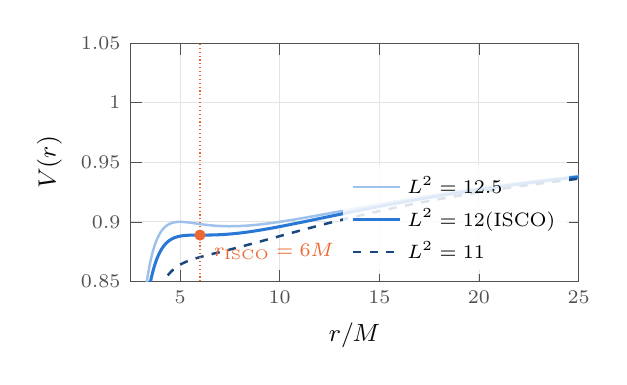
\begin{tikzpicture}
\begin{axis}[note, width=0.6\linewidth, height=0.38\linewidth, xmin=2.5, xmax=25, ymin=0.85, ymax=1.05,
  xlabel={$r/M$}, ylabel={$V(r)$}, samples=300, domain=2.5:25,
  legend style={font=\scriptsize, at={(0.98,0.03)}, anchor=south east, fill=white, fill opacity=0.85, text opacity=1, draw=none}, legend cell align=left]
  \addplot[cA!45, line width=0.9pt] {(1-2/x)*(1+12.5/x^2)}; \addlegendentry{$L^2=12.5$}
  \addplot[cA, line width=1.1pt] {(1-2/x)*(1+12/x^2)}; \addlegendentry{$L^2=12$(ISCO)}
  \addplot[cA!60!black, line width=0.9pt, dashed] {(1-2/x)*(1+11/x^2)}; \addlegendentry{$L^2=11$}
  \addplot[only marks, mark=*, mark size=1.8pt, color=cB] coordinates {(6, 0.8889)};
  \draw[cB, densely dotted] (axis cs:6,0.85) -- (axis cs:6,1.05);
  \node[font=\scriptsize, color=cB, anchor=south west] at (axis cs:6.2,0.86) {$r_\mathrm{ISCO}=6M$};
\end{axis}
\end{tikzpicture}

\caption{Schwarzschild 時空の有効ポテンシャル $V(r)$($M=1$)。$L=2\sqrt3$ で極大と極小がつながり(変曲点)、$r=6M$ が最内安定円軌道になる。}
\label{fig:veff}
\end{figure}

\subsection{等質量の合体の残骸のスピン}

\paragraph{いちばん単純な見積もり}
全質量 $M$、換算質量 $\nu M$($\nu=m_1m_2/M^2$、等質量で $\nu=1/4$)の連星が ISCO から落ち込むとする。軌道の角運動量は $\nu M\cdot L_\mathrm{ISCO}=\nu M\cdot2\sqrt3M$ なので、残骸のスピンは($M_f\simeq M$ として)
\begin{equation}
\chi_f\simeq\frac{2\sqrt3\,\nu M^2}{M^2}=2\sqrt3\,\nu=\frac{\sqrt3}{2}=0.866\quad(\nu=1/4).
\end{equation}
数値相対論の値 0.686 より大きい。比べる質量が同じくらいだと試験粒子の近似が崩れ、落ち込むあいだに重力波が角運動量を持ち去るからである。

\paragraph{数値相対論の当てはめ}
Hofmann, Barausse \& Rezzolla(\arxiv{1605.01938})は、この見積もりに $\nu$ の高次の項を足して数値相対論に合わせた。回らない親では($a_\mathrm{eff}=0$)
\begin{equation}
\chi_f=\nu\,L_\mathrm{ISCO}(0)+k_{00}\nu^2+k_{10}\nu^3,\qquad L_\mathrm{ISCO}(0)=2\sqrt3
\end{equation}
($L_\mathrm{ISCO}$ を単位質量・$M=1$ で書いた)。係数 $k_{10}=3.79245$(同論文 Table 1)と、等質量で 0.68646 になる条件から決まる $k_{00}=-3.8212$ を使うと、$\nu=1/4$ で
\begin{equation}
\chi_f=0.8660-\frac{3.8212}{16}+\frac{3.79245}{64}=0.8660-0.2388+0.0593=0.6865.
\end{equation}
単純な見積もりを、重力波で失う分だけ下げたものになっている。

\paragraph{一般の場合}
親のスピン $a_1$、$a_2$ と、それらと軌道の角運動量のなす角 $\beta$、$\gamma$、親どうしのなす角 $\alpha$ があるとき(同論文の式 13--17)、
\begin{equation}
|\bm a_f|=\frac{1}{(1+q)^2}\Bigl[a_1^2+a_2^2q^4+2a_1a_2q^2\cos\alpha+2(a_1\cos\beta+a_2q^2\cos\gamma)|\bm\ell|q+|\bm\ell|^2q^2\Bigr]^{1/2}
\end{equation}
で、$|\bm\ell|$ は上の $L_\mathrm{ISCO}$ と補正の項を $a_\mathrm{eff}$(軌道に沿ったスピンの成分の組み合わせ)で評価したものである。質量比 $q=m_2/m_1$ が小さいほど軌道の角運動量の寄与が減り、$q=1/3$ では 0.540 になる。

\subsection{2 世代目のスピンの分布}

親の質量比とスピンの分布を与え、上の式で残骸のスピンを計算した(研究ノート E10、親のスピンの向きは星団を想定して等方)。

\begin{table}[H]
\centering\small
\caption{2 世代目の生まれたときのスピン(\arxiv{1605.01938} の一般スピン版、研究ノート E10)。}
\label{tab:natal}
\begin{tabular}{@{}lcccc@{}}
\toprule
親の分布 & 中央値 & 5--95\% & $P(\chi\ge0.72)$ & $P(\chi\ge0.78)$ \\
\midrule
回らない、$q\in[0.5,1]$ & 0.675 & 0.63--0.69 & 0 & 0 \\
$a\sim\mathcal U(0,0.5)$、$q\in[0.5,1]$ & 0.676 & 0.60--0.75 & 15\% & 0.5\% \\
$a\sim\mathrm{Beta}(2,5)$、$q\in[0.5,1]$ & 0.677 & 0.59--0.76 & 18\% & 1.8\% \\
$a\sim\mathrm{Beta}(2,5)$、$q\in[0.25,1]$ & 0.657 & 0.49--0.75 & 13\% & 1.5\% \\
\bottomrule
\end{tabular}
\end{table}
2 世代目は $\chi\approx0.68$ に集中する。GW241011 の主星の観測値 $0.78\pm0.09$ は分布の上の端にあり、0.78 で生まれる確率は 2\% 以下である。

\subsection{年齢}

超放射の判定で効くのは、BH が生まれてから合体するまでの時間(年齢)である。
\begin{itemize}
\item \textbf{1 世代目}: 星が BH になってから合体するまで。古い球状星団から来る低赤方偏移の合体では、数 Gyr 以上が目安である。
\item \textbf{2 世代目}: 前の合体から次の合体まで。星団の中心に沈み、相手を見つけて連星を締めるまでの時間で、重い 2 世代目の遅れの最小値は $\sim5\times10^7$--$3\times10^8$ 年が目安である(研究ノート E9)。分布を直接示した文献はない。
\end{itemize}
2 世代目は 1 世代目より若い。この年齢の差が、自己相互作用の窓の鍵になる(\S\ref{sec:window})。

\begin{summary}
\begin{itemize}
\item Schwarzschild の ISCO は $r=6M$、$L=2\sqrt3M$。単純な見積もり $\chi_f\simeq2\sqrt3\nu=0.866$ に、重力波で失う分の補正を入れると等質量で 0.686。
\item 2 世代目の生まれたときのスピンは $\approx0.68$ に集中する(親が回っていても 95\% が 0.76 以下)。
\item 2 世代目は 1 世代目より若い。
\end{itemize}
\end{summary}

\begin{tocode}
コード: \texttt{hbr16.a\_final} が \arxiv{1605.01938} の式 16(\texttt{r\_isco}、\texttt{l\_isco}、\texttt{e\_isco} が式 2--6)。\texttt{e10\_gwonly.py} が表~\ref{tab:natal} を計算する。
\end{tocode}

% 10. 窓: すべてを組み合わせる
\section{窓: すべてを組み合わせる}\label{sec:window}

ここまでの結果を組み合わせて、研究の問い(\S\ref{sec:intro})に答える形を作る。

\subsection{二つの条件}

$\mu$ と $f$ を決めると、どの BH がどれだけ回転を失うかが決まる。窓は次の二つを同時に満たす $(\mu,f)$ である。

\paragraph{条件 1: 2 世代目は回転を保つ(上限)}
GW241011 の主星は、生まれたときのスピン $\chi_0$ から、年齢 $T_2$ のあいだに観測の下限 0.69 を下回ってはならない。回転を失う速さは $f^2$ に比例するので(式 \ref{eq:chidot_H})、これは $f$ の上限になる(式 \ref{eq:fmax})。
\begin{equation}
t_\mathrm{2G}(f)\ge T_2\quad\Longleftrightarrow\quad f\le f_\mathrm{max}.
\end{equation}

\paragraph{条件 2: 1 世代目は回転を失う(下限)}
質量とスピンの相関を超放射で説明するには、1 世代目の BH が、年齢 $T_1$ のうちに臨界スピンの近く(臨界 $+\delta$)まで回転を失わなければならない。これは $f$ の下限になる。
\begin{equation}
t_\mathrm{1G}(f)\le T_1\quad\Longleftrightarrow\quad f\ge f_\mathrm{min}(M_1).
\end{equation}
$\delta=0.18$ は、証拠を主張する解析が積み上がりに持たせた幅である。

\paragraph{両立の条件}
$f_\mathrm{min}\le f\le f_\mathrm{max}$ が空でないこと。$t\propto f^{-2}$ なので、これは年齢の比の条件と同じである。
\begin{equation}
\frac{T_1}{T_2}\ge R=\frac{t_\mathrm{1G}}{t_\mathrm{2G}}\qquad(\text{$f$ によらない、\S\ref{sec:equilibrium}}).
\end{equation}
$t\propto1/K\propto\alpha^{-5}$ なので、軽い 1 世代目ほど回転を失うのが遅く、$R$ が大きい。窓は「重い 1 世代目だけが回転を失う」形になりやすい。

\subsection{仮定の組と結果}

\begin{table}[H]
\centering\small
\caption{窓の判定に使う仮定と、$\mu=0.71\times10^{-12}\eV$ での結果(主要項の $\gamma_\mathrm{BH}$。研究ノート E9、E10)。$M_\mathrm{min}$ は 6 Gyr のうちに臨界 $+\delta$ まで回転を失える 1 世代目の最小質量($\delta=0.18/0.05$)。}
\label{tab:window}
\begin{tabularx}{\linewidth}{@{}l>{\raggedright\arraybackslash}X>{\raggedright\arraybackslash}X@{}}
\toprule
 & 楽観的な仮定 & 現実的な仮定 \\
\midrule
GW241011 の主星 & 0.78 で生まれ、年齢 $3\times10^7$ 年 & 0.72 で生まれ、年齢 $5\times10^7$ 年 \\
$f$ の上限(GW241011) & $2.4\times10^{12}\GeV$ & $1.1\times10^{12}\GeV$ \\
$M_\mathrm{min}$(GW だけ) & $8.8/10.9\Msun$ & $11.7/14.5\Msun$ \\
GRS 1915+105(付録) & 年齢 $4.5\times10^7$ 年、0.95 を保つ & 年齢 3 Gyr、0.87 を保つ \\
$M_\mathrm{min}$(GRS も入れる) & --- & $15.5/19.3\Msun$ \\
\bottomrule
\end{tabularx}
\end{table}

\begin{figure}[H]
\centering
% 窓(勉強ノート用)。データ: ../paper/figs/data/fig_window_{opt,real}.dat(研究ノート E9、paper/figs/make_fig_window.py)
\begin{tikzpicture}
\begin{groupplot}[group style={group size=2 by 1, horizontal sep=14mm},
  width=0.48\linewidth, height=0.44\linewidth, note, xmode=log, ymode=log,
  xmin=0.4e-12, xmax=1.2e-12, ymin=3e10, ymax=1e13,
  xtick={0.4e-12,0.6e-12,0.8e-12,1e-12}, xticklabels={0.4,0.6,0.8,1.0},
  xlabel={$\mu\ [10^{-12}\,\mathrm{eV}]$}]
\nextgroupplot[ylabel={$f\ [\mathrm{GeV}]$}, title={\small (a) 楽観的な仮定}]
  \fill[cB!10] (axis cs:0.60e-12,3e10) rectangle (axis cs:0.89e-12,1e13);
  \addplot[cA, line width=1.1pt] table[x=mu, y=GW241011] {../paper/figs/data/fig_window_opt.dat};
  \addplot[ink2, line width=0.8pt, densely dotted] table[x=mu, y=GRS] {../paper/figs/data/fig_window_opt.dat};
  \addplot[cC!60!black, dashed, line width=0.9pt] table[x=mu, y=M15_d18] {../paper/figs/data/fig_window_opt.dat};
  \addplot[cC, dashed, line width=0.9pt] table[x=mu, y=M20_d18] {../paper/figs/data/fig_window_opt.dat};
  \addplot[cC!45, dashed, line width=0.9pt] table[x=mu, y=M25_d18] {../paper/figs/data/fig_window_opt.dat};
  \node[font=\scriptsize, color=cA, anchor=south] at (axis cs:1.0e-12,1.4e12) {GW241011};
  \node[font=\scriptsize, color=cC!60!black, anchor=north east] at (axis cs:1.15e-12,7.5e10) {$15\Msun$};
  \node[font=\scriptsize, color=cC!80!black, anchor=north east] at (axis cs:0.90e-12,4.5e10) {$20\Msun$};
  \node[font=\scriptsize, color=cC!60, anchor=north east] at (axis cs:0.72e-12,4.5e10) {$25\Msun$};
\nextgroupplot[title={\small (b) 現実的な仮定}]
  \fill[cB!10] (axis cs:0.60e-12,3e10) rectangle (axis cs:0.89e-12,1e13);
  \addplot[cA, line width=1.1pt] table[x=mu, y=GW241011] {../paper/figs/data/fig_window_real.dat};
  \addplot[ink2, line width=0.8pt, densely dotted] table[x=mu, y=GRS] {../paper/figs/data/fig_window_real.dat};
  \addplot[cC!60!black, dashed, line width=0.9pt] table[x=mu, y=M15_d18] {../paper/figs/data/fig_window_real.dat};
  \addplot[cC, dashed, line width=0.9pt] table[x=mu, y=M20_d18] {../paper/figs/data/fig_window_real.dat};
  \addplot[cC!45, dashed, line width=0.9pt] table[x=mu, y=M25_d18] {../paper/figs/data/fig_window_real.dat};
  \node[font=\scriptsize, color=cA, anchor=south west] at (axis cs:0.41e-12,4.3e12) {GW241011};
  \node[font=\scriptsize, color=ink2, anchor=north east] at (axis cs:1.18e-12,1.35e11) {GRS(付録)};
\end{groupplot}
\end{tikzpicture}

\caption{$(\mu,f)$ 面の窓。青の実線より下で GW241011 の主星が回転を保つ(条件 1)。緑の破線より上で、その質量の 1 世代目が 6 Gyr のうちに回転を失う(条件 2、$\delta=0.18$)。灰色の点線は付録で扱う GRS 1915+105 の上限。橙の帯は証拠を主張する解析の質量(90\%)。データは論文の図(研究ノート E9)と同じ。}
\label{fig:window_study}
\end{figure}

\subsection{読み方}

\begin{itemize}
\item 楽観的な仮定では、$f\sim10^{12}\GeV$ で 10 $\Msun$ 程度より重い 1 世代目が回転を失い、GW241011 は回転を保てる。
\item 現実的な仮定では、上限が 2 倍ほど下がり、回転を失えるのは 12--15 $\Msun$ 以上の 1 世代目になる。X 線連星 GRS 1915+105 も入れると 15--19 $\Msun$ 以上。
\item 2 世代目の生まれたときのスピンは $\approx0.68$ に集中する(\S\ref{sec:secondgen})。0.78 で生まれる確率は 2\% 以下で、楽観的な仮定はその意味でかなり楽観的である。
\end{itemize}
したがって、最後に決めるのは集団解析である。問いは「GWTC-5 の質量とスピンの相関が、重い 1 世代目だけが回転を失う形を許すか」になる。

\subsection{年齢と判定の幅への依存(研究ノート E12)}

\paragraph{$f$ と年齢は縮退している}
準平衡ではスピンは $\tau=\mu(f/\Mpl)^2T$ だけで決まる(\S\ref{sec:equilibrium})。したがって GW241011 の主星からの上限は、実は $f\sqrt{T_2}$ の上限で、年齢を 4 倍にすると $f$ の上限は半分になる。上の「現実的な」$T_2=5\times10^7$ 年は、$(50+50)\Msun$ の連星の遅れの最小値の目安で、GW241011 の主星の親に近い $(10+10)\Msun$ では $3\times10^8$ 年になる。
\begin{center}\small
\begin{tabular}{rccc}
\toprule
$T_2$ [年] & 生まれたスピン & $f$ の上限 [GeV] & 回転を失う 1 世代目($\chi_0=0.7$、$\delta=0.02/0.05$)\\
\midrule
$5\times10^7$ & 0.72 & $1.1\times10^{12}$ & $16.2/14.5\Msun$ 以上\\
$3\times10^8$ & 0.72 & $4.6\times10^{11}$ & $22.4/20.1\Msun$ 以上\\
$3\times10^8$ & 0.78 & $7.6\times10^{11}$ & $18.8/16.8\Msun$ 以上\\
\bottomrule
\end{tabular}
\end{center}

\paragraph{判定の幅 $\delta$ は 0 にできない}
準平衡では臨界からのずれが $x(t)=[x_0^{-1/2}+Kt/2]^{-2}$ で近づくので(\S\ref{sec:equilibrium})、臨界 $+\delta$ に届く時間は $t=(2/K)(\delta^{-1/2}-x_0^{-1/2})$。$\delta$ が小さいと $t\simeq2/(K\sqrt\delta)$ で、$K\propto f^2$ だから、1 世代目の下限は
\begin{equation}
f_\mathrm{low}\propto\delta^{-1/4}
\end{equation}
で増える。$15\Msun$、6 Gyr、$\chi_0=0.7$ では $\delta=0.18$、0.05、0.01、0.001 で $f_\mathrm{low}=0.56$、1.0、1.7、$3.1\times10^{12}\GeV$。$\delta\to0$ では下限が GW241011 の上限を超え、窓は定義から閉じる。$\delta$ は説明のための判定で、集団解析では置かない。$\chi_\mathrm{SR}$ が予言する臨界からのずれ $x\approx4/(KT)^2\propto\alpha^{-10}f^{-4}T^{-2}$ を、そのまま測定と比べる。

\paragraph{1 世代目の自然スピン}
1 世代目の自然スピンが低い(例: Beta(0.69, 2.28))と、$10$、$15$、$20\Msun$ のうち 211 の臨界より上で生まれるのは 43、30、20\% だけである。残りは 211 の信号をそもそも持たず、一部は 322 だけが育ち、(322, 544) の固定点でゆっくり回転を失う(\S\ref{sec:three_level})。

\subsection{集団解析に渡すもの}

集団解析では、BH ごとに(質量、生まれたときのスピン、年齢)をモンテカルロで振り、$(\mu,f)$ を推定する。そのとき要る関数は、年齢 $T$ のあとのスピン
\begin{equation}
\chi_\mathrm{SR}(M,\chi_0,T;\mu,f)=\chi_T\Bigl(\alpha=GM\mu,\ \chi_0,\ \tau=\mu(f/\Mpl)^2T\Bigr)
\end{equation}
である(\S\ref{sec:equilibrium})。準平衡では三つの量だけの関数なので、表から $10^6$ 回を 1 秒以内で引ける(研究ノート E10--E12)。自由場の側($f$ が大きい)では \S\ref{sec:cloud} の飽和の扱いを使い、両者をつなぐ。

\begin{summary}
\begin{itemize}
\item 窓は「2 世代目は回転を保つ($f$ の上限)」と「1 世代目は回転を失う($f$ の下限)」の重なりで、年齢の比 $T_1/T_2\ge R$ と同じである。
\item 回転を失う速さは $\alpha^5$ に比例するので、窓では重い 1 世代目だけが回転を失う。
\item 現実的な仮定では、窓は $f\sim10^{12}\GeV$ で、回転を失うのは 12--15 $\Msun$ 以上(GW だけ)の 1 世代目。ただし $f$ の上限は $f\sqrt{T_2}$ の上限で、1 世代目の下限は判定の幅 $\delta$ に $\delta^{-1/4}$ で依存する。これを GWTC-5 の集団が許すかを、$\delta$ を使わずに集団解析で決める。
\end{itemize}
\end{summary}

\appendix
% 付録
\section{単位と数値}\label{app:units}

\begin{table}[H]
\centering\small
\caption{よく使う定数と換算。}
\label{tab:units}
\begin{tabular}{@{}lll@{}}
\toprule
量 & 値 & 使う場所 \\
\midrule
$\hbar$ & $6.582\times10^{-16}\eV\,\mathrm{s}$ & $\mu$ を振動数に直す \\
$\mu c^2/\hbar$ & $1.519\times10^{3}\,\mathrm{s}^{-1}\,(\mu/10^{-12}\eV)$ & 率の単位 \\
$GM_\odot/c^3$ & $4.925\times10^{-6}\,\mathrm{s}$ & $t_g$、$\alpha$ \\
$GM_\odot/c^2$ & $1.477\,\mathrm{km}$ & $r_g$ \\
$\alpha$ & $0.0748\,(M/10M_\odot)(\mu/10^{-12}\eV)$ & すべて \\
$\Mpl=\sqrt{\hbar c/G}$ & $2.18\times10^{-8}\,\mathrm{kg}=1.221\times10^{19}\GeV$ & $\varepsilon$、$(\Mpl/f)^4$ \\
$(M_\odot/\Mpl)^2$ & $8.35\times10^{75}$ & 粒子数の単位 $GM^2/\hbar c$ \\
1 年 & $3.156\times10^7\,\mathrm{s}$ & \\
\bottomrule
\end{tabular}
\end{table}

\paragraph{$\varepsilon$ の単位から粒子数へ}
$N=\varepsilon\,GM^2/(\hbar c)=\varepsilon\,(M/\Mpl)^2=8.35\times10^{75}\,\varepsilon\,(M/M_\odot)^2$。$M=19.6\Msun$ で $\varepsilon=1.8\times10^{-9}$(GW241011 の主星の準平衡、$f=4\times10^{12}\GeV$)なら $N=5.8\times10^{69}$。

\section{Leaver の連分数法の考え方}\label{app:leaver}

\S\ref{sec:atom} の成長率の式は $\alpha$ の小さい極限の式である。研究では、Kerr 時空の Klein--Gordon 方程式を数値的に解いて相対論的な率を出した(研究ノート E4、\texttt{research/calc/leaver.py})。考え方だけを書く。
\begin{enumerate}
\item 場を $\varphi=e^{-i\omega t+im\phi}S(\theta)R(r)$ と分けると、角度の式と動径の式に分かれる(Kerr 時空でも変数分離できる)。
\item 動径の解を、地平線で入っていくだけ、無限遠で減衰する形を先に括り出して
\[
R(r)=(r-r_+)^{-i\sigma}(r-r_-)^{i\sigma+\chi-1}e^{qr}\sum_{n=0}^\infty a_n\Bigl(\frac{r-r_+}{r-r_-}\Bigr)^n,\qquad q=-\sqrt{\mu^2-\omega^2}
\]
と置く(Dolan、\arxiv{0705.2880})。ここでの $\chi$ は Dolan の記号の指数で、スピンとは別物である。
\item 方程式に入れると、係数 $a_n$ が三項の漸化式 $\alpha_na_{n+1}+\beta_na_n+\gamma_na_{n-1}=0$ を満たす。
\item 級数が収束する(境界条件を満たす)のは、連分数の条件 $\beta_0-\alpha_0\gamma_1/(\beta_1-\alpha_1\gamma_2/(\beta_2-\cdots))=0$ を満たす $\omega$ だけである。これを複素数の $\omega$ について解くと、$\omega=E+i\Gamma$ が出る。
\end{enumerate}
研究のコードは、Dolan の表の最大成長率(6 点)を 3 桁で再現した。小さい $\alpha$ では解析式 \eqref{eq:bcst} に近づく。

\section{式と文献とコードの対応}\label{app:map}

\begin{table}[H]
\centering\small
\caption{このノートの主な式と、典拠・研究ノート・コードの対応。}
\label{tab:map}
\begin{tabularx}{\linewidth}{@{}l>{\raggedright\arraybackslash}X>{\raggedright\arraybackslash}X>{\raggedright\arraybackslash}X@{}}
\toprule
式 & 中身 & 典拠 & 研究ノート・コード \\
\midrule
\eqref{eq:chic} & 臨界スピン & 本ノートで導出 & E2、\texttt{si.chi\_threshold\_211} \\
\eqref{eq:fine} & 準位のエネルギー & \arxiv{1908.10370} 式 2.28--2.29 & \texttt{sr.omega\_over\_mu} \\
\eqref{eq:bcst} & 超放射の率(振幅) & \arxiv{1908.10370} 式 2.32--2.34 & E2、\texttt{sr.gamma\_over\_mu} \\
\eqref{eq:gammaN} & 粒子数の率 $=2\Gamma$ & 本ノート(式 2.27 から) & \texttt{sr.NORM\_N} \\
\eqref{eq:GP} & 非線形 Schr\"odinger 方程式 & 本ノートで導出(BGLS 式 12) & --- \\
\eqref{eq:gamma_SI} & 自己相互作用の率 & BGLS 式 18、21、Table V・VI & E3、\texttt{si.g\_bh}、\texttt{si.g\_inf} \\
\eqref{eq:rate211}--\eqref{eq:rateJ} & 率の方程式 & BGLS 式 34--36 & E5、\texttt{e05\_kinetics.py} \\
\eqref{eq:eq_occ} & 準平衡 & BGLS 式 55a,b(本ノートで導出) & E3、\texttt{si.eps\_eq} \\
\eqref{eq:chidot_H} & 回転を失う速さ & 本ノートで導出 & E3、E10、\texttt{si.chidot}、\texttt{chisr.H} \\
\eqref{eq:closedform} & 閉じた解 & 本ノートで導出 & --- \\
\eqref{eq:dchi_abs} & 吸収によるスピンの変化 & 本ノートで導出 & E6、E9 \\
--- & 残骸のスピン & \arxiv{1605.01938} 式 13--17 & E10、\texttt{hbr16.a\_final} \\
\bottomrule
\end{tabularx}
\end{table}


\end{document}
